
\section{Degrees when \texorpdfstring{$k\to\infty$}{k tends to infinity}: proof of Theorem~\ref{thm:degrees_hyperbolic}\label{sec:degrees}}

Since the new contribution of Theorem~\ref{thm:degrees_hyperbolic} concerns the cases where the degree $k_n \to \infty$, we 
will assume that this holds throughout this section.

\subsection{Proof overview}

We start by using the Campbell-Mecke formula to compare the degree distribution in $\GPo$ with that of the typical point in $\Ginf$. 
As we've already seen this equals 
\[
	\pmf(k) = \int_0^\infty \rho(y,k) \alpha e^{-\alpha y} \, dy.
\]
We will relate this to the Poissonized KPKVB model $\GPo$. 
More precisely, let $N_{\Po}(k)$ denote the set of degree $k$ vertices in $\GPo$. 
We then show in Section~\ref{ssec:expected_degrees_GPo} that for any $1 \ll k_n \le n -1$ with 
$k_n = \bigO{n^{\frac{1}{2\alpha + 1}}}$, $\Exp{N_{\Po}(k_n)} = (1+\smallO{1}) n \pmf(k_n)$ and more generally,

\begin{equation}\label{eq:def_factorial_moments_GPo}
	\Exp{\binom{N_{\Po}(k_n)}{r}} = (1+\smallO{1}) \frac{\Exp{N_{\Po}(k_n)}^r}{r!},
\end{equation}

\noindent
for any integer $r \ge 1$ in Section~\ref{ssec:factorial_moments_GPo}. 
The latter result requires us to analyze the joint degree distribution in $\GPo$, which we do in Section~\ref{ssec:joint_degrees_GPo}. 
The above result in particular implies concentration of $N_{\Po}(k_n)$ from which the result on the degree distribution in $\GPo$ follows for $k_n = \smallO{n^{\frac{1}{2\alpha + 1}}}$. When $k_n = (1+\smallO{1}) c n^{\frac{1}{2\alpha + 1}}$ we use the above result to show that the fraction of degree $k_n$ nodes in $\GPo$ converges to a Poisson distribution. 

To extend these results to $G_n$ we couple the construction of the KPKVB model to that of the Poissonized version $\GPo$ in Section~\ref{ssec:coupling_Gn_GPo} to show that a.a.s, $N_n(k_n) = (1+\smallO{1}) N_{\Po}(k_n)$. With these results we then prove Theorem~\ref{thm:degrees_hyperbolic} in Section~\ref{ssec:proof_thm_degrees}.

We will also establish all the above mentioned results for the finite box model $\Gbox$, since the proofs only require small 
alterations and we will need these results later on when analyzing the clustering coefficient and function.


\subsection{Expected degrees in \texorpdfstring{$\Gbox$}{G box} and \texorpdfstring{$\GPo$}{G Po}}\label{ssec:expected_degrees_GPo}

We proceed with the expected degrees in the finite box and Poissonized KPKVB model. Recall the definition of the neighbourhood balls $\BallPon{y}$ and $\BallHyp{y}$ of a point $(0,y)$ in, respectively $\Gbox$ and $\GPo$. We introduce the short hand notation
\[
	\mu_{\Po}(y) := \Mu{\BallHyp{y}} \quad \text{and} \quad \mu_{\mathrm{box}}(y) := \Mu{\BallPon{y}}.
\]

Our first results relate these measures to the measure $\mu(y)$, of the ball $\BallPo{y}$ in the infinite model $\Ginf$.

\begin{lemma}[Expected degree given height in $\GPo$]\label{lem:average_degree_P_n}
Let $\alpha > \frac{1}{2}$, $\varepsilon >0$ and $0 \leq y \leq (1-\epsilon)R$. Then as $n \to \infty$, uniformly in $y$,
\[
	\mu_{\Po}(y) = (1+\smallO{1}) \mu(y).
\]
\end{lemma}

\begin{proof}
Recall that when $y^\prime \ge R - y$ then $p^\prime \in \BallHyp{y}$ while for $y^\prime < R - y$ this is true when~\eqref{eq:def_Omega_hyperbolic} holds. We split the integral for $\mu_{Po,n}(y)$ accordingly, into two integrals $I_1$ and $I_2$,
\begin{align*}
\mu_{\Po}(y) 
&= \int_0^{R-y} 2\Phi(y,y_1)\frac{\alpha\nu}{\pi}e^{-\alpha y_1} dy_1+\int_{R-y}^R \frac{\pi n}{\nu} \frac{\alpha \nu}{\pi}e^{-\alpha y_1}dy_1 =: I_1+I_2.
\end{align*}
Firstly, we will show that the second integral $I_2=o(\mu(y))$ and then we will show that $I_1 = (1+o(1))\mu(y)$ (both with  convergence uniform in $0\leq y\leq (1-\epsilon)R$).

For the second integral $I_2$, we compute
\begin{align*}
I_2 &= \int_{R-y}^R \frac{\pi n}{\nu} \frac{\alpha \nu}{\pi}e^{-\alpha y_1}dy_1 =n(e^{-\alpha(R-y)}-e^{-\alpha R}) =ne^{-\alpha R}(e^{\alpha y} -1) =n^{1-2\alpha}\nu^{2\alpha}(e^{\alpha y} -1). 	%&= o(\xi e^{\frac{y}{2}})=o(\mu(y)).
\end{align*}
To see that $n^{1-2\alpha}\nu^{2\alpha}(e^{\alpha y} -1) = o(\mu(y))$, recall that $\mu(y)=\xi e^{\frac{y}{2}}$. So, we need to show that
\begin{align*}
\frac{n^{1-2\alpha}\nu^{2\alpha}(e^{\alpha y} -1)}{\xi e^{\frac{y}{2}}} = o(1)
\end{align*}
or equivalently that
\begin{align*}
\frac{e^{\alpha y}-1}{\xi e^{\frac{y}{2}}}=\smallO{n^{2\alpha-1}}.
\end{align*}
For this, note that
\begin{align*}
\frac{e^{\alpha y}-1}{\xi e^{\frac{y}{2}}}=\bigO{e^{\alpha y-\frac{y}{2}}} = \bigO{e^{\left(\alpha-\frac{1}{2}\right)y}}.
\end{align*}
As $y \leq (1-\epsilon)R =(1-\epsilon)2\ln \frac{n}{\nu}$ and $\alpha > \frac{1}{2}$, we have 
\[
	e^{\left(\alpha-\frac{1}{2}\right)y} \leq e^{\left(\alpha-\frac{1}{2}\right)(1-\epsilon)R} = \left(\frac{n}{\nu}\right)^{2\left(\alpha-\frac{1}{2}\right)(1-\epsilon)} = \smallO{n^{2\alpha-1}},
\]
where the convergence is uniform in $y$, $0\leq y\leq (1-\epsilon)R$, as the last upper bound does not depend on $y$.

For the first integral $I_1$, we first recall from Lemma~\ref{lem:asymptotics_Omega_hyperbolic} that there is a positive constant $K$ such that for any $\varepsilon >0$, for all $y_1, y_2 \in [0,(1-\varepsilon)R]$, $y_1+y_2 <R$, we have
\[
	e^{\frac{1}{2}(y_1+y_2)} - Ke^{\frac{3}{2}(y_1+y_2)-R} \leq \Phi(y_1,y_2) \leq e^{\frac{1}{2}(y_1+y_2)} + Ke^{\frac{3}{2}(y_1+y_2)-R}.
\]
We thus define the main and error term of $I_1$ as
\begin{align*}
I_{1,main} &=\int_0^{R-y} 2e^{\frac{y+y_1}{2}}\frac{\alpha\nu}{\pi}e^{-\alpha y_1}dy_1, \\
I_{1,error} &= \int_0^{R-y} 2Ke^{\frac{3}{2}(y+y_1)-R} \frac{\alpha\nu}{\pi} e^{-\alpha y_1} dy_1.
\end{align*}
From the error bounds for $\Phi$ as given in Lemma~\ref{lem:asymptotics_Omega_hyperbolic}, it follows that
$$I_{1,main}-I_{1,error} \leq I_1 \leq I_{1,main}+I_{1,error}. $$
We will firstly show that $I_{1,main} =(1+o(1))\mu(y) $ and then that $I_{1,error} = o(\mu(y))$.

For the main term, we obtain, as $R-y \geq \epsilon R \rightarrow \infty$, uniformly in $0\leq y\leq (1-\epsilon)R$,
\begin{align*}
I_{1,main} &= \int_0^{R-y} 2e^{\frac{y+y_1}{2}}\frac{\alpha\nu}{\pi}e^{-\alpha y_1}dy_1 
		= \frac{2\alpha\nu}{\pi}e^{\frac{y}{2}}\int_0^{R-y} e^{\left(\frac{1}{2}-\alpha\right)y_1}dy_1\\
	&=\frac{2\alpha\nu}{\pi\left(\alpha-\frac{1}{2}\right)}e^{\frac{y}{2}}
		\left(1-e^{\left(\frac{1}{2}-\alpha\right)(R-y)}\right)
		=(1+o(1))\xi e^{\frac{y}{2}} = (1+o(1))\mu(y).
\end{align*}
%\PvdH{It is not clear to the reader what the error term is. Please be specific, for example writing it out and using equation numbers.}

For the error term, we obtain, for $\alpha \not = \frac{3}{2}$, uniformly in $0\leq y\leq (1-\epsilon)R$,
\begin{align*}
I_{1,error}=\int_0^{R-y} 2Ke^{\frac{3}{2}(y+y_1)-R} \frac{\alpha\nu}{\pi} e^{-\alpha y_1} dy_1 &= 2K\frac{\alpha\nu}{\pi} e^{\frac{3}{2}y-R} \int_0^{R-y} e^{\left(\frac{3}{2}-\alpha\right)y_1}dy_1 \\
&= \frac{2K\alpha\nu}{\pi\left(\frac{3}{2}-\alpha\right)}e^{\frac{3}{2}y-R} \left(e^{\left(\frac{3}{2}-\alpha\right)(R-y)}-1\right)\\
&= \frac{2K\alpha\nu}{\pi\left(\frac{3}{2}-\alpha\right)}e^{\frac{1}{2}y} \left(e^{\left(\frac{1}{2}-\alpha\right)(R-y)}-e^{-(R-y)}\right) =o\left(\xi e^{\frac{y}{2}}\right).
\end{align*}
For the error term with $\alpha=\frac{3}{2}$, uniformly in $0\leq y\leq (1-\epsilon)R$,
\begin{align*}
\int_0^{R-y} 3Ke^{\frac{3}{2}(y+y_1)-R} \frac{\nu}{\pi} e^{-\frac{3}{2} y_1} dy_1 &= 3K\frac{\nu}{\pi} e^{\frac{3}{2}y-R} \int_0^{R-y} dy_1 = \frac{3K\nu}{\pi}e^{\frac{3}{2}y-R} (R-y) =o\left(\xi e^{\frac{y}{2}}\right).
\end{align*}
We conclude that $I_{1,error} = o(\mu(y))$ and hence $I_{1,main}\pm I_{1,error} = (1+o(1))\mu(y)$, which finishes the proof.
\end{proof}

\begin{lemma}[Expected degree given height in $\Gbox$]\label{lem:average_degree_G_box}
Let $\alpha > \frac{1}{2}$, $\varepsilon >0$ and $0 \leq y \leq (1-\epsilon)R$. Then as $n \to \infty$, uniformly in $y$,
\[
	\mu_{\mathrm{box}}(y) = (1+\smallO{1}) \mu(y).
\]
\end{lemma}

\begin{proof}
First note that since we have identified the boundaries of $[-\frac{\pi}{2}e^{\frac{R}{2}}, \frac{\pi}{2}e^{\frac{R}{2}}]$ we can assume, without loss of generality, that $p = (0,y)$. We then have that the boundaries of $\BallPon{p}$ are given by the equations $x^\prime = \pm e^{\frac{y+y^\prime}{2}}$, which intersect the left and right boundaries of $[-\frac{\pi}{2}e^{\frac{R}{2}}, \frac{\pi}{2}e^{\frac{R}{2}}]$ at height
\[
	h(y) = R + 2 \log\left(\frac{\pi}{2}\right) - y.
\]
Therefore, if $y \le 2 \log(\pi/2)$ this intersection occurs above the height $R$ of the box $\Rcal$ while in the other case the full region of the box above $h(y)$ is connected to $p$. 

We will first consider the case where $y \le 2 \log(\pi/2)$. Here we have
\begin{align*}
	\mu(\BallPon{p})
	&= \int_0^{R} \int_{-e^{\frac{y+y^\prime}{2}}}^{e^{\frac{y+y^\prime}{2}}} 
		f(x^\prime,y^\prime) \, dx^\prime \, dy^\prime\\
	&= \frac{2 \alpha \nu}{\pi} e^{\frac{y}{2}} \int_0^{R} e^{-(\alpha - \frac{1}{2})y^\prime} \, dy^\prime\\
	&= \mu(y)\left(1 - e^{-(\alpha - \frac{1}{2})R}\right),
\end{align*}
where the error term is $\smallO{1}$, uniformly in $y$.

Now let $y > 2 \log(\pi/2)$ and recall that $\mu(y) = \xi e^{\frac{y}{2}}$ where $\xi = \frac{4\alpha \nu}{(2\alpha - 1)\pi}$. Then, after some simple algebra, we have that
\begin{align*}
	\mu_{\mathrm{box}}(y)
	&= \int_0^{h(y)} \int_{-\frac{\pi}{2}e^{\frac{R}{2}}}^{\frac{\pi}{2}e^{\frac{R}{2}}} 
		\ind{|x^\prime| \le e^{\frac{y+y^\prime}{2}}} f(x^\prime,y^\prime) \, dx^\prime \, dy^\prime
		+ \int_{h(y)}^{R} \int_{-\frac{\pi}{2}e^{\frac{R}{2}}}^{\frac{\pi}{2}e^{\frac{R}{2}}} 
		f(x^\prime,y^\prime) \, dx^\prime \, dy^\prime\\
	&= \frac{2 \alpha \nu}{\pi} e^{\frac{y}{2}} \int_0^{h(y)} e^{-(\alpha - \frac{1}{2})y^\prime} \, dy^\prime
		+ \alpha \nu e^{\frac{R}{2}} \int_{h(y)}^{R} e^{-\alpha y^\prime} \, dy^\prime \\
	&= \xi e^{\frac{y}{2}}\left(1 - \left(\frac{\pi}{2}\right)^{-(2\alpha - 1)} 
		e^{-(\alpha - \frac{1}{2})(R - y)}\right)
	+ \nu e^{\frac{R}{2}}\left(\left(\frac{\pi}{2}\right)^{-2\alpha} e^{-\alpha(R - y)} 
		- e^{-\alpha R}\right)\\
	&= \mu(y)\left(1 - \phi_n(y) \right).
\end{align*}
where 
\begin{equation}\label{eq:def_average_degree_Gbox_phi}
	\phi_n(y) :=  \left(\frac{\pi}{2}\right)^{-(2\alpha - 1)} \hspace{-3pt} e^{-(\alpha - \frac{1}{2})(R - y)}
				+ \frac{\nu}{\xi}e^{-(\alpha - \frac{1}{2})R - \frac{y}{2}} - \frac{\nu}{\xi}\left(\frac{\pi}{2}\right)^{-2\alpha} e^{-(\alpha-\frac{1}{2})(R - y)}.
\end{equation}
Since $R - y \ge \varepsilon R$ we have that $|\phi_n(y)|$ is uniformly bounded by
$\bigO{e^{-(\alpha - \frac{1}{2})\varepsilon R}}$, which is $\smallO{1}$ for $\alpha > \frac{1}{2}$. 
\end{proof}

We can now use a concentration of heights argument to show that the integration of the Poisson probabilities $\Prob{\Po(\mu_{\Po}(y)) = k_n}$ over $0 \le y \le (1-\varepsilon) R$ is asymptotically equivalent to $\pmf(k_n)$. And the same holds if we instead consider $\mu_{\mathrm{box}}(y)$. The proof contains some technical elements that are contained in the Appendix to not hinder the flow of the argument. 

\begin{lemma}\label{lem:degree_integral}
Let $0 < \varepsilon < 1$. Then for all $0 \le k_n \le n - 1$, as $n \to \infty$,

\begin{equation}\label{eq:degree_integral_BallHyp}
	\int_0^{(1-\varepsilon)R} \Prob{\Po(\Mu{\BallHyp{y}} = k_n} \alpha e^{-\alpha y} \dd y
	= (1+\smallO{1}) \pmf(k_n).
\end{equation}

Moreover, the same holds if we replace $\Mu{\BallHyp{y}}$ with $\Mu{\BallPon{y}}$ in~\eqref{eq:degree_integral_BallHyp}.
\end{lemma}

\begin{proof}
We will show that
\[
	\int_0^{(1-\varepsilon)R} \Prob{\Po(\mu_{\Po}(y)) = k_n} \alpha e^{-\alpha y} \dd y
	= (1+o(1))\int_0^\infty \Pee(\Po(\xi e^{\frac{z}{2}})=k_n) \alpha e^{-\alpha z} \dd z.
\]
This implies the result because the last integral equals $(1+o(1))2\alpha \xi^{2\alpha} k_n^{-(2\alpha+1)} = (1+o(1))\pmf(k_n)$. Where the last asymptotic equality follows from~\eqref{eq:degree_distribution_P_asymptotics}.

Define the function $z(y)=2\ln\frac{\mu_{\Po}(y)}{\xi}$ (note that $z(y)$ is well-defined as $\mu_{Po,n}(y)\geq 0$ and that $z(y)$ is bijective because $\mu_{\Po}(y)$ is strictly monotone increasing and continuous, see Lemma~3.3. in \cite{gugelmann2012random}). By rearranging, we have that
\begin{align*}
\mu_{\Po}(y) = \xi e^{\frac{z(y)}{2}}.
\end{align*}
From Lemma~\ref{lem:average_degree_P_n}, it follows that uniformly for all $0\leq y\leq (1-\varepsilon)R$, $\xi e^{\frac{y}{2}} = (1+o(1))\mu_{\Po}(y) = (1+o(1))\xi e^{\frac{z(y)}{2}}$, and hence that
\begin{align*}
e^{-\alpha y} = (1+o(1))e^{-\alpha z(y)}.
\end{align*}
Next we need a similar result regarding the derivative of $\mu_{\Po}(y)$, i.e.
\[
	\mu_{\Po}^\prime(y) = (1+o(1))\frac{1}{2}\mu(y) = (1+o(1))\frac{1}{2}\mu_{\Po}(y)
	= (1+\smallO{1}) \mu^\prime(y),
\]
uniformly for $0 \leq  y \leq (1-\varepsilon)R$. This result is given by Lemma~\ref{lem:derivative_mu_Po} in the Appendix. The lemma is placed there since the proof is a straightforward though cumbersome use of function analysis and we do not want to break the flow of the argument.

We now have that
\[
	z^\prime(y) = \frac{2\mu_{\Po}^\prime(y)}{\mu_{\Po}(y)} = 1+o(1).
\]
which implies that
\begin{align*}
	\int_0^{(1-\varepsilon)R} \Prob{\Po(\mu_{\Po}(y))=k_n} \alpha e^{-\alpha y}dy 
	= (1+o(1)) \int_0^{(1-\varepsilon)R} \Prob{\Po(\xi e^{\frac{z(y)}{2}})=k_n}\alpha e^{-\alpha z(y)} z^\prime(y) dy.
\end{align*}
We now apply integration by substitution to the integral, i.e. use the new variable $z=z(y)$, to obtain 
\begin{align*}
	\int_{z(0)}^{z((1-\varepsilon)R)} \Prob{\Po(\xi e^{\frac{z}{2}})=k_n}\alpha e^{-\alpha z} dz
	= \int_{z(0)}^{z((1-\varepsilon)R)} \Prob{\Po(\mu(z))=k_n}\alpha e^{-\alpha z} dz.
\end{align*}


Note that since the function $y \mapsto 2\ln \frac{y}{\xi}$ is monotone increasing it follows that for large enough $n$, 
$\Kcal_C(k_n)\subset [z(0),z((1-\epsilon)R)]$. Therefore, by a concentration of heights argument (Proposition~\ref{prop:concentration_height_general}) it follows that
\begin{align*}
	\int_{z(0)}^{z((1-\varepsilon)R)} \Prob{\Po(\mu(z))=k_n}\alpha e^{-\alpha z} dz 
	&= (1+o(1))\int_0^\infty \Pee(Po(\mu(z))=k_n)\alpha e^{-\alpha z}dz.
\end{align*}
and hence
\[
	\int_0^{(1-\varepsilon)R} \Prob{\Po(\mu_{\Po}(y))=k_n} \alpha e^{-\alpha y}dy
	= (1+o(1))\int_0^\infty \Pee(Po(\mu(z))=k_n)\alpha e^{-\alpha z}dz,
\]
which finishes the proof for $\mu_{\Po}(y)$.

The proof for $\mu_{\mathrm{box}}(y)$ follows similar arguments. First, we define $z(y) = 2 \log (\mu_{\mathrm{box}}(y)/\xi)$ and use Lemma~\ref{lem:average_degree_G_box} instead of Lemma~\ref{lem:average_degree_P_n} to establish that $e^{-\alpha y} = (1+\smallO{1})e^{-\alpha z(y)}$. For the derivative $z^\prime(y)$ we recall from the proof of Lemma~\ref{lem:average_degree_G_box} that $\mu_{\mathrm{box}}(y) = (1 + \phi_n(y)) \mu(y)$ with $\phi_n(y)$ given by~\eqref{eq:def_average_degree_Gbox_phi}. The derivative of $\phi_n(y)$ can be uniformly bounded by $\smallO{1}$ for $0 \le y \le (1-\varepsilon)R$. Hence we get $\mu_{\mathrm{box}}^\prime(y) = (1+\smallO{1}) \mu^\prime(y)$ and thus $z^\prime(y) = 1 + \smallO{1}$ uniformly for $0 \le y \le (1-\varepsilon)R$. We can now apply the same change of variables and a concentration of heights argument to arrive at the required statement.

\end{proof}

The main result of this section now follows almost immediately.

\begin{lemma}[First moment of number of degree $k$ vertices]\label{lem:expnnkn}
Let $N_{Po}(k)$ and $\Nbox(k)$ denote the number of vertices with degree $k$ vertices in the Poissonized KPKVB model $\GPo$ and the finite box model $\Gbox$, respectively. Consider a sequence of integers $k_n\rightarrow\infty$ with $0 \leq k_n \leq n-1$.	If $k_n = O\left(n^{\frac{1}{2\alpha+1}}\right)$, then as $n \to \infty$,
\[
	\Exp{N_{Po}(k_n)} =(1+o(1)) n \pmf(k_n) \quad \text{and} \quad \Exp{\Nbox(k_n)} =(1+o(1)) n \pmf(k_n).
\]
Moreover, if $k_n \gg n^{\frac{1}{2\alpha + 1}}$ then
\[
	\Exp{N_{\Po}(k_n)} = \smallO{1} \quad \text{and} \quad \Exp{\Nbox(k_n)} = \smallO{1}.
\]
\end{lemma}

\begin{proof}
We shall consider $\GPo$. The proof of the statements for $\Gbox$ follows using the same arguments and we omit it here. 

Let $D_{\Po}(p)$ denote the degree of a node $p \in \GPo$. Then since $N_{Po}(k_n)= \sum_{v\in V(\GPo)}\1_{\{D_{\GPo}(v)=k_n\}}$ and $\Prob{D_{\Po}(p) = k}$ is invariant under translations in the $x$-axis, we can apply the Campbell-Mecke formula to obtain
\begin{align*}
	\Exp{N_{Po}(k_n)} 
	&= \int_0^R \Prob{\Po(\mu_{\Po}(y)) = k_n} \frac{\pi n}{\nu}\frac{\alpha \nu}{\pi} e^{-\alpha y}dy \\
	&=n \int_0^R \Prob{\Po(\mu_{\Po}(y)) = k_n} \alpha e^{-\alpha y}dy \\
	&=n\left( \int_0^{(1-\epsilon)R} \Prob{\Po(\mu_{\Po}(y)) = k_n} \alpha e^{-\alpha y}dy
		+ \int_{(1-\varepsilon)R}^R \Prob{\Po(\mu_{\Po}(y)) = k_n} \alpha e^{-\alpha y}dy \right),
%		\numberthis \label{eq:enpoknsplit}
\end{align*}
where $0 < \varepsilon < 1$ is a constant to be chosen later.
Note that
\begin{align*}
	\int_{(1-\varepsilon)R}^R \Prob{\Po(\mu_{\Po}(y)) = k_n}\alpha e^{-\alpha y}dy 
	\le \int_{(1-\varepsilon)R}^R \alpha e^{-\alpha y}dy 
	= \Theta(e^{-\alpha (1-\varepsilon) R}) = \Theta(n^{-2\alpha(1-\varepsilon)}) .%= o(k_n^{-(2\alpha+1)})
\end{align*}

Now first consider the case where $k_n = \bigO{n^{\frac{1}{2\alpha + 1}}}$. Then, for $\alpha > \frac{1}{2}$ and $0 < \varepsilon < \frac{1}{2\alpha} - 1$, we have $2\alpha(1-\varepsilon)>1$. Therefore, $\frac{2\alpha (1-\varepsilon)}{2\alpha+1}>\frac{1}{2\alpha+1}$ and thus
$k_n = \bigO{n^{\frac{1}{2\alpha+1}}} = \smallO{n^{\frac{2\alpha(1-\varepsilon)}{2\alpha+1}}}$. This implies that $k_n^{-(2\alpha+1)} \gg n^{-2\alpha(1-\varepsilon)}$ or, stated differently, $\Theta(n^{-2\alpha(1-\varepsilon)}) = \smallO{k_n^{-(2\alpha+1)}}$. The first statement of the lemma now follows from Lemma~\ref{lem:degree_integral}.

When $k_n \gg n^{\frac{1}{2\alpha + 1}}$, Lemma~\ref{lem:degree_integral} implies that
\[
	n \int_0^{(1-\varepsilon)R} \Pee(Po(\mu_{Po}(y))=k_n) \alpha e^{-\alpha y}dy
	= (1+\smallO{1}) n \pmf(k_n)= \bigO{n k^{-(2\alpha + 1}} = \smallO{1}.
\]
On the other hand,
\[
	n \int_{(1-\varepsilon)R}^R \Pee(Po(\mu_{Po}(y))=k_n) \alpha e^{-\alpha y}dy = \bigO{n^{1 - 2\alpha(1-\varepsilon)}}.
\]
which is $\smallO{1}$ since by our choice $2\alpha(1-\varepsilon) > 1$. Thus the second claim of the lemma follows.
\end{proof}

\subsection{Joint degrees in \texorpdfstring{$\Gbox$}{G box} and \texorpdfstring{$\GPo$}{G Po}}\label{ssec:joint_degrees_GPo}

To prove the factorization of higher moments of $N_{\Po}(k_n)$ and $\Nbox(k_n)$ as in~\eqref{eq:def_factorial_moments_GPo}, we first have to understand the joint degree distribution in $\GPo$ and $\Gbox$, respectively. This subsequently requires us to analyze the joint neighbourhoods of two points $p, p^\prime$ in these models. To explaining the proof strategy we will use the finite box model, since the formulas there are slightly easier. The results for the Poissonized KPKVB model $\GPo$ follow the same idea.

%We start with a general result for near independent Poisson random variables.
%
%\begin{lemma}\label{lem:near_independence_poisson}
%Let $k_n \to \infty$ and $X_1 = \Po(\lambda_1(n))$, $X_2 = \Po(\lambda_2(n))$ and $Y = \Po(\lambda_3(n))$, be three Poisson random variables where $\lambda_3(n) = \bigO{k_n^{1-\varepsilon}}$, for some $0 < \varepsilon < 1$ and for some $C > 0$,
%\[
%	k_n - C\sqrt{k_n \log(k_n)} \le \lambda_i(n) + \lambda_3(n) \le k_n + C\sqrt{k_n \log(k_n)},
%\] 
%for $i = 1,2$.Then, as $n \to \infty$
%\[
%	\Prob{X_1 + Y = k_n, X_2 + Y = k_n} = (1+\smallO{1}) \Prob{X_1 + Y = k_n}\Prob{X_2 + Y = k_n},
%\]
%where the error term $\smallO{1}$ only depends on $k_n, \varepsilon$ and $C$.
%\end{lemma}
%
%The proof can be found in the Appendix. To see how this lemma can be applied 

For $r\in \N$ and $p_1, \dots, p_r \in \Rcal$, we write $\Gbox\cup \{p_1,\dots,p_r\}$ for the finite box model obtained by adding $p_1,\dots,p_r$ to the vertex set of the graph and adding all corresponding edges according to the connection rule. Then we define, for any positive integer $s$ and $V \subset \{p_1,\dots,p_s\}$,
\begin{equation}\label{eq:def_joint_degree_distribution}
\varphi_{\mathrm{box}}(V, k ; p_1,\dots,p_s) = \Prob{\text{every }p\in V\text{ has degree }k\text{ in }\Gbox \cup \{p_1,\dots,p_s\}}.
\end{equation}
In particular, for two points $p, p^\prime \in \Rcal$ and $V = \{p,p^\prime\}$, $\varphi_{\mathrm{box}}(V, k ;p,p^\prime)$ is the joint degree distribution of $p, p^\prime $ in $\Gbox$. We will use similar notation for the Poissonized KPKVB model. That is, $\GPo \cup \{p_1,\dots,p_r\}$ denotes the Poissonized KPKVB model obtained by adding $p_1,\dots,p_r$ to the vertex set of the graph and adding all corresponding edges and $\varphi_{\Po}(V, k ; p_1,\dots,p_s)$ the corresponding joint degree function.

If we define,
\begin{align*}
	X_1(p,p^\prime) &:= \Po\left(\Mu{\BallPon{p}\setminus \BallPon{p^\prime}}\right),\\
	X_2(p,p^\prime) &:= \Po\left(\Mu{\BallPon{p^\prime}\setminus \BallPon{p}}\right),\\
	Y(p,p^\prime) &:= \Po\left(\Mu{\BallPon{p} \cap \BallPon{p^\prime}}\right)
\end{align*}
then each of these are independent Poisson random variables, while
\[
	\varphi_{\mathrm{box}}(\{p,p^\prime\}, k ;p,p^\prime) 
	= \Prob{X_1(p,p^\prime) + Y(p,p^\prime) = k, X_2(p,p^\prime) + Y(p,p^\prime) = k_n}.
\]
Recall the definition of $y_{k_n,C}^\pm$ from equation~\eqref{eq:def_y_k_C}. We will show (see Lemma~\ref{cor:expected_common_neighbours_Ecal_set}) that for any two points $p, p^\prime$ whose $y$-coordinate is in $\Kcal_C(k_n)$ and whose $x$-coordinates are sufficiently separated, it holds that $\Mu{\BallPon{p} \cap \BallPon{p^\prime}} = \bigO{k_n^{1-\varepsilon}}$. Since the mean of $X_1$ and $X_2$ for such two points is $k_n$, the contribution of the Poisson random variable $Y(p,p^\prime)$ to their degrees becomes negligible as $k_n \to \infty$ and hence the joint degree distribution will factorizes on this set. The main idea is that if $p$ and $p^\prime$ are sufficiently separated in the $x$-direction, then the overlap of their neighbourhoods $\BallPon{p} \cap \BallPon{p^\prime}$ is of smaller order than $\Mu{\BallPon{p}} + \Mu{\BallPon{p^\prime}}$. We now proceed with analyzing theses joint neighbourhoods.

Let $p, p^\prime \in \Rcal$ and denote by $\Ncal_{\text{box}}(p,p^\prime)$ the number of common neighbours of $p$ and $p^\prime$ in $\Gbox \cup \{p,p^\prime\}$. We shall establish an upper bound on the expected number of joint neighbours when $p$ and $p^\prime$ are sufficiently separated. Observe that $\Exp{\Ncal_{\text{box}}(p,p^\prime)} = \Mu{\BallPon{p} \cap \BallPon{p^\prime}}$. 

\begin{figure}[!t]
\centering
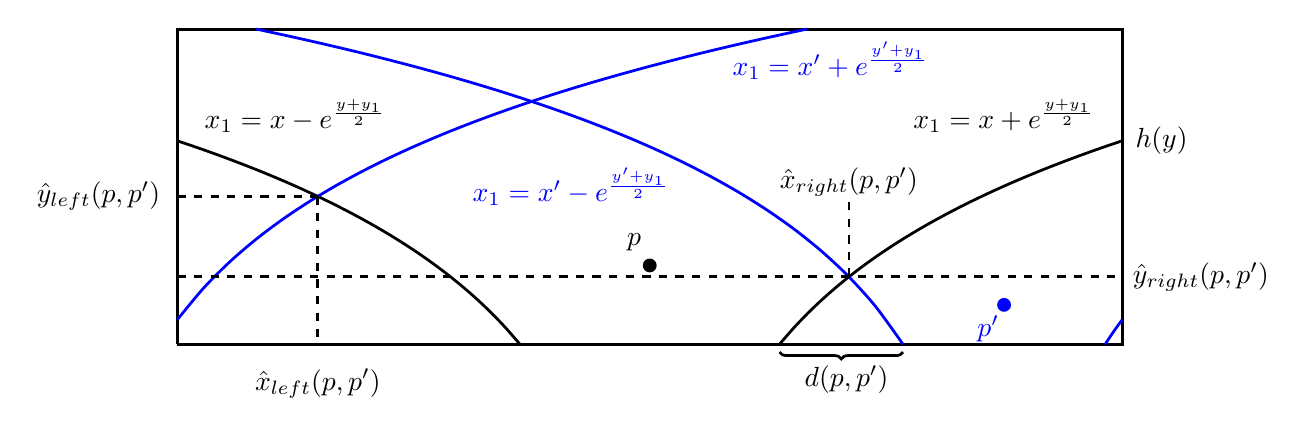
\begin{tikzpicture}
	

	\pgfmathsetmacro{\u}{0} %0
	\pgfmathsetmacro{\v}{1} %1
	\pgfmathsetmacro{\uu}{4.5} %1.4
	\pgfmathsetmacro{\vv}{0.5} %0.8
	\pgfmathsetmacro{\r}{6}
	\pgfmathsetmacro{\t}{4}
	
	%The box \Rcal
	\draw[line width=1pt] (-\r,0) -- (\r,0) -- (\r,\t) -- (-\r,\t) -- (-\r,0);
	
    \draw node[fill, circle, inner sep=0pt, minimum size=5pt] at (\u,\v) {};
    \draw node at (-0.2,1.3) {$p$};
    
    \draw node[fill,blue, circle, inner sep=0pt, minimum size=5pt] at (\uu,\vv) {};
    \draw node at (4.3,0.2) {\color{blue}$p^\prime$};
	
	\draw[domain=1.6487:6,smooth,variable=\x,black,line width=1pt] plot (\x, {2*ln(\x)-1});
    \draw[domain=-1.6487:-6,smooth,variable=\x,black,line width=1pt] plot (\x, {2*ln(-\x)-1});
    \draw[domain=5.7840:6,smooth,variable=\x,blue,line width=1pt] plot (\x, {2*ln(\x-4.5)-0.5});
    \draw[domain=3.2160:-5,smooth,variable=\x,blue,line width=1pt] plot (\x, {2*ln(4.5-\x)-0.5});
    \draw[domain=2:-6,smooth,variable=\x,blue,line width=1pt] plot (\x, {2*ln(\x+7.5)-0.5});
    
    
    
    \draw [decorate,decoration={brace},line width=1pt] (3.2160,-0.1) -- (1.6487,-0.1);
    \draw node at (2.5,-0.45) {$d(p,p^\prime)$};
    
%    \draw [dotted,line width=1pt] (2.5298,0.8563) -- (2.5298,1.7);
%    \draw node at (2.5298,2) {$\hat{x}(p,p^\prime)$};
    
    %Define intersection left black and shifted blue curve
    \pgfmathsetmacro{\vast}{2*ln((2*\r - \uu)/(exp(\v/2) + exp(\vv/2)))}
    \pgfmathsetmacro{\uast}{(\uu - 2*\r)/(1+exp((\vv-\v)/2))}
    %Define intersection right black and left blue curve
    \pgfmathsetmacro{\vvast}{2*ln((\uu)/(exp(\v/2) + exp(\vv/2)))}
    \pgfmathsetmacro{\uuast}{(\u*exp(\vv/2) + \uu*exp(\v/2))/(exp(\v/2) + exp(\vv/2))}
    \pgfmathsetmacro{\h}{2*ln(\r)-\v}
%    \draw[dotted,thick,black] (4.5208,2.0174) -- (4.5208,0);
%    \draw[dotted,thick,black] (4.5208,2.0174) -- (6,2.0174);
    
%    \draw node at (4.5208,-0.5) {$w_x(p,p^\prime)$};
%    \draw node at (7,2.0174) {$w_y(p,p^\prime)$};
    
    \draw node at (\r+0.5,\h) {$h(y)$};
    
    \draw node at (2.3,3.6) {\color{blue}$x_1 = x^\prime + e^{\frac{y^\prime + y_1}{2}}$};
    \draw node at (-1,2) {\color{blue}$x_1 = x^\prime - e^{\frac{y^\prime + y_1}{2}}$};
    \draw node at (-4.5,2.9) {$x_1 = x - e^{\frac{y + y_1}{2}}$};
    \draw node at (4.5,2.9) {$x_1 = x + e^{\frac{y + y_1}{2}}$};
	
	
	\draw[dashed,black,line width=1pt] (-\r,\vast) -- (\uast,\vast);
	\draw node at (-\r-1,\vast) {\color{black}$\hat{y}_{\text{left}}(p,p^\prime)$};
	\draw[dashed,line width=1pt] (\uast,\vast) -- (\uast,0);
	\draw node at (\uast,-0.5) {$\hat{x}_{\text{left}}(p,p^\prime)$};

	\draw[dashed,black,line width=1pt] (-\r,\vvast) -- (\r,\vvast);
	\draw node at (\r+1,\vvast) {\color{black}$\hat{y}_{\text{right}}(p,p^\prime)$};
	\draw[dashed,line width=1pt] (\uuast,\vvast) -- (\uuast,\vvast+1);
	\draw node at (\uuast,\vvast+1.2) {$\hat{x}_{\text{right}}(p,p^\prime)$};
	
	
\end{tikzpicture}
\caption{Schematic representation of the neighbourhoods of $p$ and $p^\prime$ in $\Gbox$ when $|x - x^\prime| > e^{\frac{y}{2}} + e^{\frac{y^\prime}{2}}$ used for the proof of Lemma \ref{lem:common_neighbours_Pcal_n}. Note that although here $p^\prime \notin \BallPon{p}$, this is not true in general. This situation was merely chosen to improve readability of the figure.}
\label{fig:representation_disjoint_neighbourhoods_P_n_3}
\end{figure}


We start by analyzing the shape of the joint neighbourhood. Due to symmetry and the fact that we have identified the left and right boundaries of the box $\Rcal$, we can, without loss of generality, assume that $p = (0,y)$ and $p^\prime = (x^\prime,y^\prime)$ with $x^\prime > 0$. To understand the computation it is helpful to have a picture. Figure~\ref{fig:representation_disjoint_neighbourhoods_P_n_3} shows such an example. There are several different quantities that are important. The first are the heights where the left and right boundaries of the ball $\BallPon{p}$ hit the boundaries of the box $\Rcal$. Since $x = 0$ these heights are the same and we denote their common value by $h(y)$. We also need to know the coordinates $\hat{y}_{\text{right}}(p,p^\prime)$ and $\hat{x}_{\text{right}}(p,p^\prime)$ of the intersection of the right boundary of the neighbourhood of $p$ with the left boundary of the neighbourhood of $p^\prime$ and those for the intersection of the left boundary of the neighbourhood of $p$ with the right boundary of the neighbourhood of $p^\prime$, which we denote by $\hat{y}_{\text{left}}(p,p^\prime)$ and $\hat{x}_{\text{left}}(p,p^\prime)$. Finally we will denote by $d(p,p^\prime)$ the distance between the lower right boundary of $\BallPon{p}$ and the lower left of $\BallPon{p^\prime}$, which is positive only when the bottom parts of both neighbourhoods do not intersect, as is the case in Figure~\ref{fig:representation_disjoint_neighbourhoods_P_n_3}. The condition $d(p,p^\prime) > 0$ is exactly the right notion for $p$ and $p^\prime$ being sufficiently separated.

We start by deriving expressions for these important coordinates. For this we introduce some notation. For any $p = (x,y) \in \Rcal$ we will define the left and right boundary functions as, respectively,
\begin{align}
	b_p^-(z) &= \begin{cases}
		2 \log\left(x-z\right) - y &\mbox{if }  -\frac{\pi}{2} e^{R/2} \le z \le x - e^{y/2}  \\
		2\log\left(\pi e^{R/2} + x - z\right) - y 
			&\mbox{if } x - e^{(y + R)/2} + \pi e^{R/2} \le z \le \frac{\pi}{2} e^{R/2}\\
		0 &\mbox{otherwise}
	\end{cases} \label{eq:def_left_boundary_Bp} \\ 
	b_p^+(z) &= \begin{cases}
		2 \log\left(z-x\right) - y &\mbox{if } x + e^{y/2} \le z \le \frac{\pi}{2} e^{R/2} \\
		2\log\left(\pi e^{R/2} + z - x\right) - y 
			&\mbox{if } -\frac{\pi}{2} e^{R/2} \le z \le x + e^{(y + R)/2} - \pi e^{R/2}\\
		0 &\mbox{otherwise}
	\end{cases}
\end{align}
Note that these functions describe the boundaries of the ball $\BallPon{p}$. In particular, $p^\prime = (x^\prime, y^\prime) \in \BallPon{p}$ if and only if $y^\prime \ge \min\left\{b_p^-(x^\prime), b_p^+(x^\prime)\right\}$.

We shall derive the expressions for the point $(\hat{x}_{\text{left}}(p,p^\prime), \hat{y}_{\text{left}}(p,p^\prime))$. The $x$-coordinate $\hat{x}_{\text{left}}(p,p^\prime)$ is the solution to the equation $b_{p}^+(z) = b_{p^\prime}^-(z)$ for $-\frac{\pi}{2} e^{R/2} \le z \le + e^{y/2}$. This equation becomes
\[
	2\log\left(\pi e^{R/2} + z - x^\prime\right) - y^\prime = 2 \log\left(x^\prime-z\right) - y^\prime,
\]
whose solution is $\frac{x^\prime - \pi e^{R/2}}{1 + e^{(y^\prime - y)/2}}$. Plugging this into either the left or right hand side of the above equation yields the $y$-coordinate $\hat{y}_{\text{left}}(p,p^\prime) = 2 \log\left(\frac{\pi e^{R/2} - x^\prime}{e^{y/2} + e^{y^\prime/2}}\right)$. The expressions for $\hat{x}_{\text{right}}(p,p^\prime$ and $\hat{y}_{\text{right}}(p,p^\prime)$ are derived in a similar way. The expression for $d(p,p^\prime)$ follows as the difference $b_{p^\prime}^-(x^\prime - e^{y^\prime/2}) - b_p^+(e^{y/2})$.

The full expressions of all coordinates are given below for further reference.

\begin{align}
	h(y) &= R - y + 2\log\left(\frac{\pi}{2}\right) \label{eq:def_height_y_P_n}\\
%	h_1(p^\prime) &= 2\log\left(x^\prime + \frac{\pi}{2}e^{\frac{R}{2}}\right) - y^\prime \label{eq:def_height_left_P_n} \\
%	h_2(p^\prime) &= 2\log\left(\frac{\pi}{2}e^{\frac{R}{2}} - x^\prime\right) - y^\prime 
%		\label{eq:def_height_right_P_n} \\
%	\iota_x(p,p^\prime) &= \frac{(x^\prime-x)e^{\frac{y}{2}}}{e^{\frac{y}{2}} - e^{\frac{y^\prime}{2}}}
%		\label{eq:def_x_intersection_close_boundaries}\\
%	\iota_y(p,p^\prime) &= 2\log\left(\frac{x^\prime - x}{e^{\frac{y}{2}} - e^{\frac{y^\prime}{2}}}\right)
%		\label{eq:def_y_intersection_close_boundaries}\\
	\hat{y}_{\text{right}}(p,p^\prime) &= 2\log\left(\frac{x^\prime}{e^{\frac{y}{2}} + e^{\frac{y^\prime}{2}}}\right)\\
	\hat{x}_{\text{right}}(p,p^\prime) &= \frac{x^\prime}{1 + 	
		e^{\frac{y^\prime - y}{2}}},\\
	\hat{y}_{\text{left}}(p,p^\prime) &= 2 \log\left(\frac{\pi e^{R/2} - x^\prime}{e^{\frac{y}{2}} + e^{\frac{y^\prime}{2}}}\right),\\
	\hat{x}_{\text{left}}(p,p^\prime) &= \frac{x^\prime - \pi e^{R/2}}{1 + e^{\frac{y^\prime - y}{2}}}, \\
	d(p,p^\prime) &= |x - x^\prime|_n - \left(e^{\frac{y}{2}} + e^{\frac{y^\prime}{2}}\right).
	\label{eq:def_d_p_p_prime}
\end{align}

The following result shows that if $d(p,p^\prime) > 0$, then the expected number of common neighbours is $\smallO{\Mu{\BallPon{p}} + \Mu{\BallPon{p^\prime}}}$.

\begin{lemma}\label{lem:common_neighbours_Pcal_n}
Let $p, p^\prime \in \Rcal$. Then, whenever $|x - x^\prime|_n > \left(e^{\frac{y}{2}} + e^{\frac{y^\prime}{2}}\right)$,
\[
	\Exp{\Ncal_{\text{box}}(p,p^\prime)} \le \Mu{\BallPon{p}}
	\left(\left(\frac{|x - x^\prime|}{e^{\frac{y}{2}} + e^{\frac{y^\prime}{2}}}\right)^{-(2\alpha - 1)}  
	+ \frac{\nu}{\xi} e^{-(\alpha - \frac{1}{2})(R-y)}\right).
\]
\end{lemma}

\begin{proof}
Again, without loss of generality we assume that $p = p_0 = (0,y)$ and $p^\prime = (x^\prime, y^\prime)$ with $0 \le x^\prime \le \frac{\pi}{2} e^{R/2}$. Note that since $0 < x^\prime \le \frac{\pi}{2} e^{R/2}$, $ \hat{y}_{\mathrm{right}}(p,p^\prime) \le \hat{y}_{\mathrm{left}}(p,p^\prime)$. We write $\hat{y}$ for $\hat{y}_{\mathrm{right}}(p,p^\prime)$ and observe that below $\hat{y}$ the balls $\BallPon{p}$ and $\BallPon{p^\prime}$ are disjoint. Therefore, if we define $A := \left\{p_1 = (x_1,y_1) \in \Rcal \cap \BallPon{p} \, : \, y_1 \ge \hat{y} \right\}$. Then
\[
	\Exp{\Ncal_{\text{box}}(p,p^\prime)} \le \Mu{A}.
\]
We proceed with computing the right hand side
\begin{align*}
	\Mu{A} &= \int_{\hat{y}}^{h(y)} 
		\int_{- e^{\frac{y + y_1}{2}}}^{e^{\frac{y^\prime+y_1}{2}}} 
		f(x_1,y_1) \dd x_1 \dd y_1
		+ \int_{h(y)}^{R} \int_{-\frac{\pi}{2}e^{R/2}}^{\frac{\pi}{2} e^{R/2}} 
		\hspace{-10pt}  f(x_1,y_1) \dd x_1 \dd y_1 \\
	&= \frac{2\alpha \nu}{\pi}e^{\frac{y}{2}}
		\int_{\hat{y}}^{h(y)} e^{-(\alpha - \frac{1}{2})y_1} \dd y_1 
		+ \alpha \nu e^{R/2} \int_{h(y)}^R e^{-\alpha y_1} \dd y_1\\
	&\le \xi\left(e^{\frac{y}{2}} + e^{\frac{y^\prime}{2}}\right) e^{-(\alpha-\frac{1}{2})\hat{y}}
		+ \nu e^{R/2} e^{-\alpha h(y)} \\
	&= \Mu{\BallPon{p}}\left(
		e^{-(\alpha-\frac{1}{2})\hat{y}} + \frac{\nu}{\xi} e^{-(\alpha - \frac{1}{2})(R-y)}\right).
\end{align*}
The result follows by plugging in 
\[
	\hat{y} := \hat{y}_{\text{right}}(p,p^\prime) = 2 \log\left(\frac{x^\prime}{e^{\frac{y}{2}} + e^{\frac{y^\prime}{2}}}\right),
\]
and noting that $x^\prime$ is the same as $|x - x^\prime|$, by our generalization step.

\end{proof} 

We can also prove a similar result for the Poissonized KPKVB model $\GPo$, denoting by $\Ncal_{\Po}(p,p^\prime)$ the number of joint neighbours in $\GPo \cup \{p,p^\prime\}$.

\begin{lemma}\label{lem:common_neighbours_KPKVB}
Let $0 < \varepsilon < 1$, $p, p^\prime \in \Rcal$ with $y,y^\prime \le (1-\varepsilon)R$, denote by $\Ncal_{\Po}(p,p^\prime)$ the number of joint neighbours of $p, p^\prime$ in $\GPo$ and let $K$ be the constant from Lemma~\ref{lem:asymptotics_Omega_hyperbolic}. Then, whenever $|x - x^\prime|_n > \left(e^{\frac{y}{2}} + e^{\frac{y^\prime}{2}}\right)\left(1 + \frac{\pi^2 K}{4}\right)$,
\[
	\Exp{\Ncal_{\Po}(p,p^\prime)} \le \Mu{\BallHyp{p}}
	\left(e^{(2\alpha - 1)\lambda} \left(\frac{|x - x^\prime|}{e^{\frac{y}{2}} + e^{\frac{y^\prime}{2}}}\right)^{-(2\alpha - 1)}  
	+ \frac{\nu}{\xi} e^{-(\alpha - \frac{1}{2})(R-y)}\right),
\]
where
\[
	\lambda = \log\left(1 + \frac{\pi^2 K}{4}\right).
\]
\end{lemma}

\begin{proof}
We will proceed in a similar fashion as for Lemma~\ref{lem:common_neighbours_Pcal_n}. That is, we will bound the expected number of common neighbours by the number of neighbors of $p$ whose $y$-coordinate is above the intersection of the right boundary of $\BallHyp{p}$ and the left boundary of $\BallHyp{p^\prime}$. Denote by $\hat{y}$ the height of this intersection point. Then
\begin{align*}
	\Exp{\Ncal_{\Po}(p,p^\prime)} &\le \frac{2\alpha \nu}{\pi} \int_{\hat{y}}^{R-y} \Phi(y,y_1) e^{-\alpha y_1} \dd y_1
		+ \alpha \nu e^{R/2} \int_{R-y}^{R} e^{-\alpha y_1} \dd y_1.
\end{align*} 
The second integral is bounded by $\frac{\nu}{\xi} \Mu{\BallPon{y}} e^{-(\alpha - \frac{1}{2})(R-y)}$. We bound the first integral using Lemma~\ref{lem:asymptotics_Omega_hyperbolic} as
\begin{align*}
	\frac{2\alpha \nu}{\pi} \int_{\hat{y}}^{R-y} \Phi(y,y_1) e^{-\alpha y_1} \dd y_1
	&\le \frac{2\alpha \nu}{\pi} \int_{\hat{y}}^{R-y} \left(e^{\frac{y+y_1}{2}} + K e^{\frac{3}{2}(y + y_1)-R}\right) 
		e^{-\alpha y_1} \dd y_1 \\
	&\le \frac{2\alpha \nu}{\pi} (1+K)e^{\frac{y}{2}} \int_{\hat{y}}^{R-y} e^{-(\alpha - \frac{1}{2}) y_1} \dd y_1\\
	&\le (1 + K)\Mu{\BallPon{p}}  e^{-(\alpha - \frac{1}{2})\hat{y}},
\end{align*}
where we used that $\frac{3y_1}{2} \le R - y + \frac{y_1}{2}$ for all $y_1 \le R-y$ for the second line. 

It remains to compute $\hat{y}$, for which we will establish the following bound
\begin{equation}\label{eq:joint_neighbors_KPKVB_intersection}
	\hat{y} \ge 2 \log\left(\frac{x^\prime}{e^{\frac{y}{2}} + e^{\frac{y^\prime}{2}}}\right) - 2\lambda.
\end{equation}

To show~\eqref{eq:joint_neighbors_KPKVB_intersection} we note that for any point $y_1 \ge \hat{y}$, the corresponding $x$-coordinate of the left boundary of $\BallHyp{p^\prime}$ must be to the left of that of the ball $\BallHyp{p}$, i.e.
$x^\prime - \Phi(y^\prime, y_1) \le \Phi(y,y_1)$. Therefore it is enough to show that for all 
\[
	y_1 \le 2 \log\left(\frac{x^\prime}{e^{\frac{y}{2}} + e^{\frac{y^\prime}{2}}}\right) - 2\lambda
\]
it holds that $\Phi(y,y_1) \le x^\prime - \Phi(y^\prime, y_1)$, with $\lambda$ as defined in the statement of the lemma. Note that by assumption on $x^\prime := |x - x^\prime|_n$ (since we can take $x = 0$) the above upper bound is non-negative. Using Lemma~\ref{lem:asymptotics_Omega_hyperbolic} it suffices to prove that for all such $y_1$,
\[
	e^{\frac{y + y_1}{2}} + K e^{\frac{3}{2}(y + y_1) - R} \le x^\prime - e^{\frac{y^\prime + y_1}{2}}
	- K e^{\frac{3}{2}(y^\prime + y_1) - R},
\]
which is equivalent to
\[
	\left(e^{\frac{y}{2}} + e^{\frac{y^\prime}{2}}\right) e^{\frac{y_1}{2}} 
	+ K e^{-R} \left(e^{\frac{y}{2}} + e^{\frac{y^\prime}{2}}\right)^3 e^{\frac{3 y_1}{2}} \le x^\prime.
\]
Plugging the upper bound for $y_1$ into the left hand side and using that $(e^{y/2} + e^{y^\prime/2})^3 \ge e^{3y/2} + e^{3y^\prime/2}$, we obtain
\begin{align*}
	\left(e^{\frac{y}{2}} + e^{\frac{y^\prime}{2}}\right) e^{\frac{y_1}{2}} 
		+ K e^{-R} \left(e^{\frac{y}{2}} + e^{\frac{y^\prime}{2}}\right)^3 e^{\frac{3 y_1}{2}}
	&\le x^\prime e^{-\lambda} + K e^{-R} (x^\prime)^3 e^{-3\lambda}
		\le x^\prime \left(e^{-\lambda} + \frac{\pi^2 K}{4} e^{-3\lambda}\right)\\
	&\le x^\prime e^{-\lambda} \left(1 + \frac{\pi^2 K}{4}\right) = x^\prime,
\end{align*} 
where we also used that $x^\prime \le \frac{\pi}{2} e^{-R/2}$.
\end{proof}

Let us now define the \emph{stripe}
\begin{equation}\label{eq:def_stripe}
	\stripknc = \Rcal \cap (\R_+ \times \Kcal_C(k_n)).
\end{equation} 
and in addition define, for any $0 < \varepsilon < 1$, the following set
\begin{equation}\label{eq:def_joint_degree_set_E_growing_k}
	\mathcal{E}_{\varepsilon}(k_n) = \left\{(p,p^\prime) \in \stripknc
		\, : \,  |x - x^\prime|_n > k_n^{1 + \varepsilon} \right\}, 
\end{equation}
where $|x|_n = \min\{|x|, \pi e^{R/2} - |x|\}$ denotes the norm on the finite box $\Rcal$ where the left and right boundaries are identified. Then for any two points $p,p^\prime \in \mathcal{E}_\varepsilon(k_n)$ the expected number of joint neighbours is $\smallO{k_n}$.

\begin{lemma}\label{cor:expected_common_neighbours_Ecal_set}
Fix $0 < \varepsilon < 1$ and let $\varepsilon^\prime = \min\{\varepsilon(2\alpha - 1),\varepsilon\}$. Then for all $(p,p^\prime) \in \mathcal{E}_\varepsilon(k_n)$, as $n \to \infty$,
\[
	\Mu{\BallPon{p} \cap \BallPon{p^\prime}} = \bigO{k_n^{1-\varepsilon^\prime}}.
\] 
\end{lemma}

\begin{proof}
Since for all $(p,p^\prime) \in \mathcal{E}_\varepsilon(k_n)$ we have $\Mu{\BallPon{p}}, \Mu{\BallPon{p^\prime}} = \bigT{k_n}$, Lemma~\ref{lem:common_neighbours_Pcal_n} implies that
\[
	\Mu{\BallPon{p} \cap \BallPon{p^\prime}} \le \bigO{k_n} \phi_n(p,p^\prime),
\]
where
\[
	\phi_n(p,p^\prime) = 2\left(\frac{|x - x^\prime|_n}{e^{\frac{y}{2}} + e^{\frac{y^\prime}{2}}}\right)^{-(2\alpha - 1)} 
		+ \frac{3 \nu^{2\alpha + 1}e^{-(\alpha - \frac{1}{2})R} e^{\alpha y}}{2 \pi^{2\alpha}\left(
		e^{\frac{y}{2}} + e^{\frac{y^\prime}{2}}\right)}
		+ \frac{\nu e^{-(\alpha - \frac{1}{2})R}}{e^{\frac{y}{2}} + e^{\frac{y^\prime}{2}}}. 
\]
We thus need to show that $\phi_n(p,p^\prime) = \bigO{k_n^{-\varepsilon^\prime}}$. For $(p,p^\prime) \in \mathcal{E}_\varepsilon(k_n)$, it holds that $e^{y/2}, e^{y^\prime/2} = \bigT{k_n}$ and $|x - x^\prime|_n > k_n^{1+\varepsilon}$ and hence
\begin{align*}
	 2\left(\frac{|x - x^\prime|_n}{e^{\frac{y}{2}} + e^{\frac{y^\prime}{2}}}\right)^{-(2\alpha - 1)}
	 =	\bigO{k_n^{-\varepsilon(2\alpha - 1)}}.
\end{align*}
For the second term in $\phi_n(p,p^\prime)$ we use that $e^{\alpha y^\ast} = \bigT{k_n^{2\alpha}}$ and $e^{R} = \bigT{n^2}$ to obtain
\[
	\frac{3 \nu^{2\alpha + 1}e^{-(\alpha - \frac{1}{2})R} e^{\alpha y}}{2 \pi^{2\alpha}\left(
			e^{\frac{y}{2}} + e^{\frac{y^\prime}{2}}\right)}
	= \bigO{1} n^{-(2\alpha - 1)} k_n^{2\alpha - 1} = \bigO{n^{-(\alpha - \frac{1}{2})}}.
\]
Finally, the third term satisfies $\bigO{n^{-(2\alpha - 1)}k_n^{-1}}$, and we conclude that
\[
	\phi_n(p,p^\prime) = \bigO{k_n^{-\varepsilon(2\alpha - 1)} + n^{-(\alpha - \frac{1}{2})}
	+ n^{-(2\alpha - 1)}k_n^{-1}} = \bigO{k_n^{-\varepsilon^\prime}},
\]
where we used that $\varepsilon^\prime = \min\{\varepsilon(2\alpha - 1),\varepsilon\}$. 
\end{proof}

It is clear that using Lemma~\ref{lem:common_neighbours_KPKVB} instead of Lemma~\ref{lem:common_neighbours_Pcal_n}, the above proof applies to the Poissonized KPKVB model, yielding the following result.

\begin{lemma}\label{cor:expected_common_neighbours_KPKVB}
Fix $0 < \varepsilon < 1$ and let $\varepsilon^\prime = \min\{\varepsilon(2\alpha - 1),\varepsilon\}$. Then for all $(p,p^\prime) \in \mathcal{E}_\varepsilon(k_n)$, as $n \to \infty$,
\[
	\Mu{\BallHyp{p} \cap \BallHyp{p^\prime}} = \bigO{k_n^{1-\varepsilon^\prime}}.
\] 
\end{lemma}

Recall the definition of the stripe $\stripknc = \Rcal \cap (\R_+ \times [y_{k_n,C}^-, y_{k_n,C}^+])$ from~\eqref{eq:def_stripe}. Consider a fixed number of points $p_1, \dots, p_r$. Then, if their $x$-coordinates are sufficient far apart and their $y$ coordinates lie within the stripe $\stripknc$, their degrees are asymptotically independent.

\begin{lemma}[Asymptotic factorization of degree probabilities]\label{lem:probdegFact}
Let $(k_n)$ be a sequence of integers with $0\leq k_n \leq n-1$, $k_n = \bigO{n^{\frac{1}{2\alpha+1}}}$ and $k_n \rightarrow \infty$.
Let $C, C^\prime>0$ and $r,s$ be positive integers with $r+1\leq s$. Fix $0<\varepsilon<1$. Then, it holds uniformly for all $(v_1,\dots,v_s) \in \left(\stripknc\right)^{s} = \stripknc \times \dots \times \stripknc$, satisfying $|x_{v_i}-x_{v_{r+1}}|\geq k_n^{1+\varepsilon}$ for all  $1\leq i \leq r$,  that
\[
	\varphi(\{v_1,\dots,v_{r+1}\};v_1,\dots,v_s)
	=(1+o(1))\varphi(\{v_1,\dots,v_r\};v_1,\dots,v_s)\varphi(\{v_{r+1}\};v_1,\dots,v_s)+\bigO{k_n^{-C^\prime}},
\]
where $\varphi$ is either $\varphi_{\Po}$ or $\varphi_{\mathrm{box}}$.
(Here uniformity means that the $\smallO{1}$ and $\bigO{k_n}$ terms do not depend on $v_1,\dots,v_{s}$.)
\end{lemma}

\begin{proof}
Let $H=\GPo \cup\{p_1,\dots,p_s\}$ or $H=\Gbox \cup \{p_1,\dots,p_s\}$ and $1\leq r\leq s$. For $1\leq j \leq r$, let $Y_j$ be the number of vertices of $H$ which are adjacent to both $p_j$ and $p_{r+1}$. Let $X_j$ be the number of vertices of $H$ which are adjacent to $p_j$, but not to $p_{r+1}$. Then, $X_j+Y_j= D_{H}(p_j)$ is the degree of $p_j$ in $H$. 

Now let $X_{r+1}$ be the number of vertices of $H$ which are adjacent to $p_{r+1}$, but to none of $p_1,\dots,p_r$. Let $Y_{r+1}$ be the number of vertices of $H$ which are adjacent to $p_{r+1}$, and at least one of $p_1,\dots,p_r$. Then, $X_{r+1}+Y_{r+1}=D_H(p_{r+1})$ is the degree of $p_{r+1}$ in $H$. By definition, we therefore have
\begin{align*}
\varphi(\{p_1,\dots,p_{r+1}\};p_1,\dots,p_s)&=\Prob{X_1+Y_1=\dots=X_{r+1}+Y_{r+1}=k_n}, \\
\varphi(\{p_1,\dots,p_r\};p_1,\dots,p_s)&=\Prob{X_1+Y_1=\dots=X_r+Y_r=k_n}, \\
\varphi(\{p_{r+1}\};p_1,\dots,p_s)&=\Prob{X_{r+1}+Y_{r+1}=k_n},
\end{align*}
and the claim of the lemma is that
\begin{equation}\label{eq:probdegfact_main}
	\begin{aligned}
		&\Prob{X_1+Y_1=\dots=X_{r+1}+Y_{r+1}=k_n} \\
		&= (1+o(1))\Prob{X_1+Y_1=\dots=X_r+Y_r=k_n}\Prob{X_{r+1}+Y_{r+1}=k_n}+\bigO{k_n^{-C}}.
	\end{aligned}
\end{equation}

To prove~\eqref{eq:probdegfact_main} let $\varepsilon'=\min(\varepsilon,\varepsilon(2\alpha-1))\in (0,1)$. Since for $1\leq i \leq r$, it is given that $|x_{p_i}-x_{p_{r+1}}|\geq k_n^{1+\varepsilon}$, then in the case where $H = \GPo \cup\{p_1,\dots,p_s\}$ it follows from Lemma~\ref{lem:common_neighbours_KPKVB} that $\E[Y_j] = \bigO{k_n^{1-\varepsilon'}}$. When $H=\Gbox \cup \{p_1,\dots,p_s\}$ we get the same result using Lemma~\ref{lem:common_neighbours_Pcal_n}. The rest of the proof is independent of which of the two models we consider and only uses that $\E[Y_j] = \bigO{k_n^{1-\varepsilon'}}$.

As $Y_{r+1} \leq Y_1+\dots+Y_r$, we also have $\mu:=\Exp{Y_{r+1}} = \bigO{k_n^{1-\varepsilon'}}$. In particular, there is $c_0>0$ such that $c_0\sqrt{k_n^{1-\varepsilon'}\ln k_n^{1-\varepsilon'}}\geq c_1\sqrt{\mu\ln\mu}$ (where $c_1=\sqrt{\frac{2C}{1-\varepsilon'}}$, which is well-defined because $1-\varepsilon'>0$). Now define
\begin{align*}
A_n=[\mu-c_0\sqrt{k_n^{1-\varepsilon'}\ln k_n^{1-\varepsilon'}},\mu+c_0\sqrt{k_n^{1-\varepsilon'}\ln k_n^{1-\varepsilon'}}]\cap \N_0.%=[\mu-c\sqrt{\mu\ln \mu},\mu+c\sqrt{\mu\ln \mu}].
\end{align*}
By equation~\eqref{eq:def_chernoff_bound_poisson_C}, we have
\begin{align*}
	\Prob{Y_{r+1} \not \in A_n} 
	&= \Prob{|Y_{r+1}-\mu|\geq c_0\sqrt{k_n^{1-\varepsilon'}\ln k_n^{1-\varepsilon'}}}\\
	&\le \Prob{|Y_{r+1}-\mu|\geq c_1\sqrt{\mu\ln\mu}}
	=\bigO{k_n^{-\frac{(1-\varepsilon')c_1^2}{2}}}.
\end{align*}
As by definition $c_1$ satisfies $\frac{(1-\varepsilon')c_1^2}{2}=C$, this implies that for the event $S_n = \{Y_{r+1}\in A_n\}$,
\[
	\Prob{S_n^c}=\bigO{k_n^{-C}}.
\]
Beginning with the left-hand side of the claim of the lemma, the law of total probability applied to the events $\{Y_{r+1}=y_{r+1}\}$, for all $y_{r+1}\in A_n$, and $S_n^c$ implies that
\begin{align*}
	&\Prob{X_1+Y_1=\dots=X_{r+1}+Y_{r+1}=k_n} \\
	&=\sum_{y_{r+1}\in A_n} \Prob{X_1+Y_1=\dots=X_{r+1}+y_{r+1}=k_n|Y_{r+1}=y_{r+1}}\Prob{Y_{r+1}=y_{r+1}}\\ 
	&\hspace{10pt}+ \Prob{X_1+Y_1=\dots=X_{r+1}+Y_{r+1}=k_n|S_n^c} \Prob{S_n^c}\\
	&=\sum_{y_{r+1}\in A_n} \Prob{X_1+Y_1=\dots=X_{r+1}+y_{r+1}=k_n|Y_{r+1}=y_{r+1}} 
		\Prob{Y_{r+1}=y_{r+1}}+\bigO{k_n^{-C}}.
\end{align*}
As $X_{r+1}$ is independent of $X_1, \dots, X_r, Y_1, \dots, Y_r$ by the properties of a Poisson process (as $X_{r+1}$ counts the number of points in a set which is disjoint of $X_1,\dots,X_r, Y_1, \dots, Y_r$), it follows that
\begin{align*}%\label{eq:afterindep}
	&\Prob{X_1+Y_1=\dots=X_{r+1}+Y_{r+1}=k_n} \\
	&=\sum_{y_{r+1} \in A_n} \Prob{X_1+Y_1=\dots=X_{r}+Y_r=k_n|Y_{r+1}=y_{r+1}}
		\Prob{X_{r+1}+y_{r+1}=k_n} \Prob{Y_{r+1}=y_{r+1}}\\
	&\hspace{10pt} +\bigO{k_n^{-C}}.
\end{align*}
We will now show that uniformly for all $y_{r+1}, s \in A_n$, it holds that,
\begin{align}\label{eq:yrp1tos}
	\Prob{X_{r+1}=k_n-y_{r+1}} = (1+o(1))\Prob{X_{r+1}=k_n-s}.
\end{align}
To see this, observe that for all $y_{r+1},s\in A_n$, we have that $|y_{r+1}-s|\leq 2c\sqrt{k_n^{1-\varepsilon'}\ln k_n^{1-\varepsilon'}}$. Denote the expectation of $X_{r+1}$ by $\lambda$, write $\delta_n = k_n-y_{r+1}-\lambda$ and note that
\begin{align*}
	\frac{\Prob{X_{r+1}=k_n-y_{r+1}}}{\Prob{X_{r+1}=k_n-s}} 
	&= \frac{\Prob{X_{r+1}=k_n-y_{r+1}}}{\Prob{X_{r+1}=k_n-y_{r+1}+(y_{r+1}-s)}}\\
	&=\frac{(k_n-y_{r+1}+(y_{r+1}-s))!}{(k_n-y_{r+1})!}\lambda^{s-y_{r+1}}
\end{align*}
We will now use that $\frac{(a+b)!}{a!} = (1+o(1))(a+b)^b$ for $b^2=o(a)$, applied to $a=k_n-y_{r+1}$ and $b=y_{r+1}-s$. To see this auxiliary fact, note that by Stirling's approximation to the factorial (see e.g.~\cite{Dutkay2013},~\cite{Nanjundiah1959}), it follows that
\begin{align*}
	\frac{(a+b)!}{a!}=(1+o(1))\frac{(a+b)^{a+b+\frac{1}{2}}e^{-a-b}}{a^{a+\frac{1}{2}}e^{-a}}
	=(1+o(1))\left(1+\frac{b}{a}\right)^{a+\frac{1}{2}}(a+b)^b e^{-b}.
\end{align*}
Since $1+\frac{b}{a}\leq e^{\frac{b}{a}}$, it holds that $(1+\frac{b}{a})^a \leq e^b$. Furthermore, as $\ln(1+x)\geq x-\frac{x^2}{2}$ (for $x\in (-1,1)$), we have that $(1+\frac{b}{a})^a =e^{a\ln(1+\frac{b}{a})}\geq e^{a(\frac{b}{a}-\frac{b^2}{2a})} =e^{b-\frac{b^2}{2a}}=(1+o(1))e^{b}$ because $b^2=o(a)$. Finally, $b^2=o(a)$ also implies that $(1+\frac{b}{a})^\frac{1}{2}=1+o(1)$. This finishes the proof of the auxiliary fact and we can continue with
\begin{align*}
	\frac{\Prob{X_{r+1}=k_n-y_{r+1}}}{\Prob{X_{r+1}=k_n-s}}
	&=(1+o(1)) (k_n-y_{r+1}+(y_{r+1}-s))^{y_{r+1}-s} \lambda^{s-y_{r+1}} \\
	&=(1+o(1)) (\lambda+\delta_n+(y_{r+1}-s))^{y_{r+1}-s} \lambda^{s-y_{r+1}} \\
	&=(1+o(1))\left(1+\frac{\delta_n+(y_{r+1}-s)}{\lambda}\right)^{y_{r+1}-s} \\
	&=(1+o(1)) e^{\frac{\delta_n(y_{r+1}-s)}{\lambda}} e^{\frac{(y_{r+1}-s)^2}{\lambda}} = 1+o(1),
\end{align*}
where the last line follows since $\delta_n, |y_{r+1}-s| \leq 2c_0\sqrt{k_n^{1-\varepsilon'}\ln k_n^{1-\varepsilon'}}$ and $\lambda=\Theta(k_n)$ and therefore, with convergence uniform in $y_{r+1},s$,
\[
	\frac{\delta_n(y_{r+1}-s)}{\lambda}, \frac{(y_{r+1}-s)^2}{\lambda} \leq \frac{4c_0^2 k_n^{1-\varepsilon'}\ln k_n^{1-\varepsilon'}}{\lambda}  \rightarrow 0.
\]
As $\Prob{S_n^c}=\bigO{k_n^{-C}}$, we have
\begin{align*}
	1=\sum_{s\in A_n}\Prob{Y_{r+1}=s}+\bigO{k_n^{-C}}.
\end{align*}
From~\eqref{eq:yrp1tos}, it then follows that
\begin{align*}
	\Prob{X_{r+1}=k_n-y_{r+1}} 
	&=\Prob{X_{r+1}=k_n-y_{r+1}} \sum_{s\in A_n} \Prob{Y_{r+1}=s}+\bigO{k_n^{-C}}\\
	&= (1+o(1)) \sum_{s\in A_n} \Prob{Y_{r+1}=s} \Prob{X_{r+1}=k_n-s}+\bigO{k_n^{-C}} \\
	&=(1+o(1))\sum_{s\in A_n} \Prob{X_{r+1}+Y_{r+1}=k_n, Y_{r+1}=s}+\bigO{k_n^{-C}} \\
	&=(1+o(1))\Prob{X_{r+1}+Y_{r+1}=k_n, Y_{r+1}\in A_n}+\bigO{k_n^{-C}} \\
	&=(1+o(1))\left(\Prob{X_{r+1}+Y_{r+1}=k_n}-\Prob{X_{r+1}+Y_{r+1}=k_n, Y_{r+1}\not \in A_n}\right)+\bigO{k_n^{-C}} \\
	&=(1+o(1))\Prob{X_{r+1}+Y_{r+1}=k_n}+\bigO{k_n^{-C}}.
\end{align*}
Note that $\Prob{X_{r+1}+Y_{r+1}=k_n}$ no longer depends on $y_{r+1}$ and neither does the $\bigO{k_n^{-C}}$ error term. Therefore we have
\begin{align*}
	&\Prob{X_1+Y_1=\dots=X_{r+1}+Y_{r+1}=k_n} \\
	&\sum_{y_{r+1} \in A_n} \Prob{X_1+Y_1=\dots=X_{r}+Y_r=k_n|Y_{r+1}=y_{r+1}} 	
		\Prob{X_{r+1}+y_{r+1}=k_n}\Prob{Y_{r+1}=y_{r+1}}+\bigO{k_n^{-C}}\\
	&=(1+o(1))\Prob{X_{r+1}+Y_{r+1}=k_n}\sum_{y_{r+1} \in A_n} 	
		\Prob{X_1+Y_1=\dots=X_{r}+Y_r=k_n|Y_{r+1}=y_{r+1}}\Prob{Y_{r+1}=y_{r+1}}\\
	&\hspace{10pt}+\bigO{k_n^{-C}}.
\end{align*}
For the last summation we have
\begin{align*}
	&\sum_{y_{r+1} \in A_n} \Prob{X_1+Y_1=\dots=X_{r}+Y_r=k_n|Y_{r+1}=y_{r+1}}\Prob{Y_{r+1}=y_{r+1}} \\
	&= \Prob{X_1+Y_1=\dots=X_r+Y_r=k_n,Y_{r+1}\in A_n} \\
	&= (1+o(1))\Prob{X_1+Y_1=\dots=X_r+Y_r=k_n}+\bigO{k_n^{-C}}.
\end{align*}
Finally, plugging this into the previous step gives 
\begin{align*}
	&\Prob{X_1+Y_1=\dots=X_{r+1}+Y_{r+1}=k_n} \\
	&=(1+o(1))\Prob{X_{r+1}+Y_{r+1}=k_n}\sum_{y_{r+1} \in A_n} 	
		\Prob{X_1+Y_1=\dots=X_{r}+Y_r=k_n|Y_{r+1}=y_{r+1}}\Prob{Y_{r+1}=y_{r+1}}\\
	&\hspace{10pt}+\bigO{k_n^{-C}} \\
	&=(1+o(1))\Prob{X_{r+1}+Y_{r+1}=k_n}\Prob{X_1+Y_1=\dots=X_r+Y_r=k_n}+\bigO{k_n^{-C}}.
\end{align*}
which establishes~\eqref{eq:probdegfact_main} and thus the claim of the lemma.
\end{proof}

\subsection{Factorial moments of degrees}\label{ssec:factorial_moments_GPo}

Now that we have analyzed the joint neighbourhoods and degree distributions in both the Poissonized KPKVB and finite box model, we can show convergence of the factorial moments of the number of nodes of degree $k$ in both models.

\begin{lemma}[Factorial moments]\label{lem:factmoment}
Recall that $N_{Po}(k)$ denotes the number of degree $k$ vertices in $\GPo$. Let $(k_n)$ be a sequence of integers with $0\leq k_n \leq n-1$, $k_n = \bigO{n^{\frac{1}{2\alpha+1}}}$ and $k_n \rightarrow \infty$. Then, for any positive integer $r$, it holds that
\[
	\Exp{{N_{Po}(k_n) \choose r}} =(1+o(1)) \frac{(\Exp{ N_{Po}(k_n)})^r}{r!}.
\]
\end{lemma}

The proof of this result requires the following technical lemma which states that the integration of the joint degree distribution can be factorized.

\begin{lemma}[Factorization of degrees]
	\label{lem:asympind}
	Let $(k_n)$ be a sequence of integers with $0\leq k_n \leq n-1$, $k_n = \bigO{n^{\frac{1}{2\alpha+1}}}$ and $k_n \rightarrow \infty$.
	
	Let $\varphi$ be either $\varphi_{\mathrm{box}}$ or $\varphi_{\Po}$. Then we have that
	\begin{align*}
	&\int_\Rcal \cdots \int_\Rcal \varphi(\{p_1,\dots,p_r \}, k_n ;p_1,\dots,p_r) 
		 \dd \mu(p_1) \cdots \dd \mu(p_r) \\
	&= (1+o(1))\left(\int_\Rcal  \varphi(\{p_1\}, k_n ;p_1) \dd \mu(p)\right)^r .
	\end{align*}
\end{lemma}

\begin{proof}
Let $C>r(2\alpha+1)$ and define the set $A = (\Rcal \times \cdots \times\Rcal) \backslash (\stripknc \times \cdots\times \stripknc)$. We will first show that the contribution of the integration of $\varphi$ over this range is negligible. 

For $(p_1,\dots,p_r) \in (\Rcal \times \cdots \times\Rcal) \backslash (\stripknc \times \cdots\times \stripknc)$, there is a $j$, $1\leq j\leq r$, such that $y_j \not \in [y_{k_n,c}^-,y_{k_n,c}^+]$, so that the Chernoff bound (see in~\ref{eq:chernoff_bound_degrees}) yields that $\Prob{D_{\GPo}(v_j)=k_n } = \bigO{k_n^{-C}}$. As, for $1\leq j\leq r$, the event $\{D_{\GPo}(p_1)=\dots=D_{\GPo}(p_r)=k_n\}$ implies the event $\{D_{\GPo}(v_j)=k_n\}$, it follows that $\Prob{D_{\GPo}(p_1)=\dots=D_{\GPo}(p_r)=k_n} = \bigO{k_n^{-C}}$ and hence,
\begin{align*}
	\int_A \Pee(D_{\GPo}(p_1)=\dots=D_{\GPo}(p_r)=k_n) \dd \mu(p_1) \cdots \dd \mu(p_r)	= O\left(n^r k_n^{-C}\right).
\end{align*}

Next we note that by the concentration of heights (Proposition~\ref{prop:concentration_height_general}) it follows that
\begin{align*}
	\int_{\stripknc} \varphi(\{p_1\}, k_n ;p_1) \dd \mu(p_1) 
	&= (1+\smallO{1}) \int_\Rcal  \varphi(\{p_1\}, k_n ;p_1) \dd \mu(p_1) \\
	&= (1+\smallO{1}) 2\alpha \xi^{2\alpha} n k_n^{-(2\alpha + 1)} \numberthis \label{eq:integration_average_degree_stripe}
\end{align*}
Since for $C>r(2\alpha+1)$ it holds that $n^r k_n^{-C} = \smallO{\left(n k_n^{-(2\alpha + 1)}\right)^r}$ it now suffices to show that
\begin{align*}
	&\int_{\stripknc} \cdots \int_{\stripknc} \varphi(\{p_1,\dots,p_r \}, k_n ;p_1,\dots,p_r) 
		\dd \mu(p_1)\cdots \dd \mu(p_r) \\
	&= (1+o(1))\left(\int_{\stripknc}  \varphi(\{p_1\}, k_n ;p_1) \dd \mu(p_1) \right)^r.
\end{align*}

We will prove this using induction. More precisely, for every fixed positive integer $s$, we will show by induction on $r$, $1\leq r\leq s$, that for all $p_{r+1},\dots,p_s \in \stripknc$, it holds that
\begin{align*}
	&\int_{\stripknc} \cdots \int_{\stripknc} \varphi(\{p_1,\dots,p_r\}, k_n ;p_1,\dots,p_s)
		\dd \mu(p_1) \cdots \dd \mu(p_r)\\
	&= (1+o(1))\left(\int_{\stripknc} \varphi(\{p_1\}, k_n ;p_1) \dd \mu(p_1)\right)^r .
\end{align*}
Note that for $r=s$ this is the claim of the lemma. Throughout the proof $H$ is either $\GPo \cup\{p_1,\dots,p_s\}$ or $\Gbox \cup \{p_1,\dots,p_s\}$, depending on whether $\varphi$ is, respectively, $\varphi_{\Po}$ or $\varphi_{\mathrm{box}}$.

For $r=1$, we only need to show that uniformly for $p_1 \in \stripknc$,
\begin{align*}
\varphi(\{p_1\}, k_n ;p_1,\dots,p_s) = (1+o(1))\varphi(\{p_1\}, k_n ;p_1).
\end{align*}
To see this, note that as $p_1\in \stripknc$, the expected degree of $p_1$ in $\GPo$ is $\Theta(k_n)$. Assume that $p_1$ is adjacent to $s'<s$ many vertices among $p_2,\dots,p_s$. Then, as $s'<s$ is bounded and $k_n \rightarrow \infty$ as $n\rightarrow \infty$,  we have that
\begin{align*}
\Pee(D_{\GPo}(p_1)=k_n-s') = (1+o(1))\Pee(D_{\GPo}(p_1)=k_n).
\end{align*}
So, we have the base case of the induction,
\begin{align*}
\varphi(\{p_1\}, k_n ;p_1,\dots,p_s)&=\Pee(D_H(p_1)=k_n)
= \Pee(D_{\GPo}(p_1)=k_n-s')\\
&= (1+o(1))\Pee(D_{\GPo}(p_1)=k_n)=(1+o(1))\varphi(\{p_1\}, k_n ;p_1).
\end{align*}
Assuming the claim holds for integer $r <s$, we will show that it holds for $r+1$.

Let $p_{r+2},\dots,p_s\in \stripknc$ (if $r+2>s$, this definition is void and the corresponding points will never be used in the proof).
Fix $0<\epsilon<1$ small enough s.t. $\frac{1}{2}+\epsilon<\alpha$. Define the region that the $(r+1)$-th vertex $p_{r+1}$ is far apart from all other vertices horizontally,
$$\Fcal_\epsilon(k_n)=\{(p_1,\dots,p_{r+1}) \in \left(\stripknc\right)^{r+1}: \forall 1\leq i \leq r: |x_{p_i}-x_{p_{r+1}}|\geq k_n^{1+\epsilon}\}.$$

We will split the integration into this region and its complement $\Fcal_\epsilon(k_n)^c = \left(\stripknc\right)^{r+1} \backslash \Fcal_\epsilon(k_n)$.

Firstly, we derive an upper bound for the complement $\Fcal_\epsilon(k_n)^c$. Note that 
\[
	\varphi(\{p_1,\dots,p_{r+1}\}, k_n ;p_1,\dots,p_s) \leq \varphi(\{p_1,\dots,p_r\}, k_n ;p_1,\dots,p_s),
\]
and so,
\begin{align*}
	&\int \int_{\Fcal_\epsilon(k_n)^c} \varphi(\{p_1,\dots,p_{r+1}\}, k_n ;p_1,\dots,p_s)
		\dd \mu(p_1) \cdots \dd \mu(p_{r+1})\\
	&\leq \int \int_{\Fcal_\epsilon(k_n)^c} \varphi(\{p_1,\dots,p_r\}, k_n ;p_1,\dots,p_s)
		\dd \mu(p_1) \cdots \dd \mu(p_{r+1}).
\end{align*}

For $(p_1,\dots,p_{r+1})\in \Fcal_\epsilon(k_n)^c$, we have that $(p_1,\dots,p_r) \in \left(\stripknc\right)^r$ and $p_{r+1}=(x_{r+1},y_{r+1})$ satisfies $y_{k_n,c}^-\leq y_{r+1}\leq y_{k_n,c}^+$ and $x_{r+1}$ falls into an interval $I_n$ of length $2k_n^{1+\epsilon}$.
As the integrand $\varphi(\{p_1,\dots,p_r\};p_1,\dots,p_s)$ is constant in $x_{r+1}$, we can upper bound the corresponding integration as follows,
\begin{align*}
	&\int_{\{(x_{r+1},y_{r+1})\in\stripknc: x_{r+1}\in I_n\}} \varphi(\{p_1,\dots,p_r\}, k_n ;p_1,\dots,p_s) 
		\dd \mu(p_{r+1}) \\
	&= \int_{y_{k_n,c}^-}^{y_{k_n,c}^+} \int_{I_n} \varphi(\{p_1,\dots,p_r\}, k_n ;p_1,\dots,p_s)\frac{\alpha \nu}{\pi} e^{-\alpha y_{r+1}} dx_{r+1}dy_{r+1} \\
	&\leq 2k_n^{1+\epsilon} \varphi(\{p_1,\dots,p_r\}, k_n ;p_1,\dots,p_s)\int_{y_{k_n,c}^-}^{y_{k_n,c}^+}  \frac{\alpha \nu}{\pi} e^{-\alpha y_{r+1}} dy_{r+1}.
\end{align*}
Furthermore, we have that
\begin{align*}
	\int_{y_{k_n,c}^-}^{y_{k_n,c}^+} e^{-\alpha y_{r+1}}dy_{r+1} 
	\leq \int_{y_{k_n,c}^-}^\infty e^{-\alpha y_{r+1}}dy_{r+1} 
	= \bigO{e^{-\alpha y_{k_n,c}^-}} = \bigO{\left( \frac{k_n-c\sqrt{k_n\ln k_n}}{\xi}\right)^{-2\alpha}} 
	= \bigO{k_n^{-2\alpha}}.
\end{align*}
We have thus established that
\begin{align*}
	&\int \int_{\Fcal_\epsilon(k_n)^c} \varphi(\{p_1,\dots,p_r\}, k_n ;p_1,\dots,p_s)
		\dd \mu(p_1) \cdots \dd \mu(p_{r+1})\\
	&\leq \bigO{k_n^{1+\epsilon} k_n^{-2\alpha}}\int_{\stripknc} \cdots \int_{\stripknc} 
		\varphi(\{p_1,\dots,p_r\}, k_n ;p_1,\dots,p_s) \dd \mu(p_1) \cdots \dd \mu(p_{r}).
\end{align*}
The $r$-fold integral can the bounded from above using the induction hypothesis as
\begin{align}\label{eq:indhyp}
	\bigO{k_n^{1+\epsilon-2\alpha}}\left(\int_{\stripknc} \varphi(\{p_1\};p_1) \dd \mu(p_1) \right)^r .
\end{align}
Finally, we use that $k_n^{1+\epsilon-2\alpha} = \smallO{\int_{\stripknc} \varphi(\{p_1\};p_1)\mu_n(dp_1)}$. To see this, we will firstly show that $k_n^{1+\epsilon-2\alpha} = \smallO{nk_n^{-(2\alpha+1)}}$ and then apply~\eqref{eq:integration_average_degree_stripe}, which says that
\begin{align*}
\int_{\stripknc} \varphi(\{p_1\};p_1) \dd \mu(p_1) = \bigT{n k_n^{-(2\alpha+1)}}.
\end{align*}
By our choice of $\epsilon$, we have that $\frac{1}{2}+\epsilon<\alpha$, which implies that $\frac{2+\epsilon}{1+2\alpha}<1$, and hence, using $k_n = \bigO{n^{\frac{1}{2\alpha+1}}}$,
\begin{align*}
\frac{k_n^{1+\epsilon-2\alpha}}{nk_n^{-(2\alpha+1)}} = n^{-1} k_n^{2+\epsilon} = \bigO{n^{-1} n^{\frac{2+\epsilon}{1+2\alpha}}} = \smallO{n^{-1}n}= \smallO{1}.
\end{align*}
Having shown that $k_n^{1+\epsilon-2\alpha} = \smallO{\int_{\stripknc} \varphi(\{p_1\};p_1)\mu_n(dp_1)}$, we therefore conclude from~\eqref{eq:indhyp} that
\begin{align*}
	&\int \int_{\Fcal_\epsilon(k_n)^c} \varphi(\{p_1,\dots,p_r\}, k_n ;p_1,\dots,p_s)
		\dd \mu(p_1) \cdots \dd \mu(p_{r+1})\\
	&=\smallO{\int_{\stripknc} \varphi(\{p_1\}, k_n ;p_1)\mu_n(dp_1)}
		\left(\int_{\stripknc} \varphi(\{p_1\}, k_n ;p_1) \dd \mu(p_1) \right)^r  \\
	&=\smallO{\left(\int_{\stripknc} \varphi(\{p_1\}, k_n ;p_1) \dd \mu(p_1)\right)^{r+1}}.
\end{align*}

For the integration over $\Fcal_\epsilon(k_n)$, recall that by Lemma~\ref{lem:probdegFact}, \[
	\varphi(\{p_1,\dots,p_{r+1}\}, k_n ;p_1,\dots,p_s)
	=(1+o(1))\varphi(\{p_1,\dots,p_r\}, k_n ;p_1,\dots,p_s)
	\varphi(\{p_{r+1}\}, k_n ;p_1,\dots,p_s)+\bigO{k_n^{-C}}.
\]
This implies that
\begin{align*}
	&\int \int_{\Fcal_\epsilon(k_n)} \varphi(\{p_1,\dots,p_{r+1}\}, k_n ;p_1,\dots,p_s) 
		 \dd \mu(p_1) \cdots \dd \mu(p_{r+1})\\
	&=(1+o(1))\int \int_{\Fcal_\epsilon(k_n)} \varphi(\{p_1,\dots,p_r\}, k_n ;p_1,\dots,p_s) 
		\varphi(\{p_{r+1}\};p_1,\dots,p_s) \dd \mu(p_1) \cdots \dd \mu(p_{r+1}) \\
	&\hspace{10pt}+\bigO{k_n^{-C}}\int \int_{\Fcal_\epsilon(k_n)} 
		\dd \mu(p_1) \cdots \dd \mu(p_{r+1}) =:M+E.
\end{align*}
To finish the induction step we have to show that
\begin{align*}
M=(1+o(1)) \left(\int_{\stripknc} \varphi(\{p_1\}, k_n ;p_1)\mu_n(dp_1)\right)^{r+1}
\end{align*}
and
\begin{align*}
E=\smallO{\left(\int_{\stripknc} \varphi(\{p_1\}, k_n ;p_1)\mu_n(dp_1)\right)^{r+1}}.
\end{align*}

For $M$, note that we can factorize to integration over $p_1,\dots,p_r$ and over $p_{r+1}$.

Furthermore, we note that the condition $(p_1,\dots,p_{r+1})\in \Fcal_\epsilon(k_n)$ implies that (writing $p_{r+1}=(x_{r+1},y_{r+1})$) the horizontal coordinate $x_{r+1}$ falls into an interval $I_n$ of length $L_n$, satisfying
\[
	\frac{\pi n}{\nu}-2rk_n^{1+\epsilon}\leq L_n\leq \frac{\pi n}{\nu}-2k_n^{1+\epsilon}.
\]
As $k_n^{1+\epsilon} = \bigO{n^{\frac{1+\epsilon}{2\alpha+1}}} = o(n)$ for $\epsilon<1$ and $\alpha>\frac{1}{2}$, this shows that the length of the integration range in $x_{r+1}$ satisfies $L_n=(1+o(1))\frac{\pi n}{\nu}$. Thus, we have that
\begin{align*}
	M &= (1+o(1))\int_{I_n}\int_{y_{k_n,c}^-}^{y_{k_n,c}^+} \varphi(\{p_{r+1}\}, k_n ;p_1,\dots,p_s)
		\frac{\alpha\nu}{\pi} e^{-\alpha y_{r+1}}dy_{r+1}dx_{r+1}\\
	&\hspace{15pt} \times \int_{\stripknc} \cdots \int_{\stripknc} 
		\varphi(\{p_1,\dots,p_r\}, k_n ;p_1,\dots,p_s) \dd \mu(p_1) \cdots \dd \mu(p_{r})\\
	&=(1+o(1))n\int_{y_{k_n,c}^-}^{y_{k_n,c}^+} \varphi(\{p_{r+1}\}, k_n ;p_1,\dots,p_s)\alpha e^{-\alpha y_{r+1}}dy_{r+1}\\
	&\hspace{15pt} \times \int_{\stripknc} \cdots \int_{\stripknc} \varphi(\{p_1,\dots,p_r\};p_1,\dots,p_s)
		\dd \mu(p_1) \cdots \dd \mu(p_{r})\\
	&=(1+o(1))\int_{\stripknc} \varphi(\{p_{r+1}\}, k_n ;p_1,\dots,p_s)\mu_n(dp_1)\\
	&\hspace{15pt} \times\int_{\stripknc} \cdots \int_{\stripknc} \varphi(\{p_1,\dots,p_r\}, k_n ;p_1,\dots,p_s)
		\dd \mu(p_1) \cdots \dd \mu(p_{r}).
\end{align*}
By applying the base case of the induction to the first factor and the induction hypothesis to the second one, we have derived that
\begin{align*}
M&=(1+o(1))\left(\int_{\stripknc} \varphi(\{p_1\}, k_n ;p_1) \dd \mu(p_1) \right)^{r+1}.
\end{align*}
Finally, for $E$ we observe that
\begin{align*}
	E=\bigO{k_n^{-C}}\int \int_{\Fcal_\epsilon(k_n)} \dd \mu(p_1) \cdots \dd \mu(p_{r+1}) = \bigO{k_n^{-C}}(1+o(1))n^{r+1}.
\end{align*}
Recall that again by~\eqref{eq:integration_average_degree_stripe},
\begin{align*}
\int_{\stripknc} \varphi(\{p_1\}, k_n ;p_1) \dd \mu(p_1) = \bigT{n k_n^{-(2\alpha+1)}},
\end{align*}
which implies that
\begin{align*}
\left(\int_{\stripknc} \varphi(\{p_1\}, k_n ;p_1) \dd \mu(p_1) \right)^{r+1} 
= \bigT{n^{r+1}k_n^{-r(2\alpha+1)}}.
\end{align*}
For $C>r(2\alpha+1)$, we can conclude that indeed
\begin{align*}
E = \bigO{n^{r+1}k_n^{-C}}=\smallO{n^{r+1}k_n^{-r(2\alpha+1)}}=\smallO{\left(\int_{\stripknc} \varphi(\{p_1\}, k_n ;p_1) \dd \mu(p_1)\right)^{r+1}}.
\end{align*}
\end{proof}

We now prove the result for the factorial moments.

\begin{proofof}{Lemma~\ref{lem:factmoment}}
We give the proof for the Poissonized KPKVB model. The proof for the finite box model $\Gbox$ follows using similar arguments.

First of all, we observe that
\begin{align*}
{N_{\Po}(k_n) \choose r} = \frac{1}{r!} \sum_{p_1,\dots,p_r\in V(\GPo), \atop \text{distinct}} \1_{\{D_{\GPo}(p_1)=\dots=D_{\GPo}(p_r)=k_n\}}.
\end{align*}
This can be seen by induction on $r$. For $r=1$, the claim is clear. Assuming it holds for $r\geq 1$, by the induction hypothesis,
\begin{align*}
&{N_{\Po}(k_n) \choose r+1} = {N_{\Po}(k_n) \choose r} \frac{N_{\Po}(k_n)-r}{r+1} \\
&= \frac{1}{(r+1)!}\sum_{p_1,\dots,p_r\in V(\GPo), \atop \text{distinct}} \1_{\{D_{\GPo}(p_1)=\dots=D_{\GPo}(p_r)=k_n\}} (N_{\Po}(k_n)-r).
\end{align*}
Now, we can write
\[
	N_{\Po}(k_n) = \sum_{\stackrel{p_{r+1} \in V(\GPo),}{p_{r+1} \not \in\{ p_1,\dots,p_r\}} } \1_{\{D_{\GPo}(p_{r+1})=k_n\}}+\sum_{p_{r+1} \in \{p_1,\dots,p_r\}}\1_{\{D_{\GPo}(p_{r+1})=k_n\}}.
\]
The first sum leads to the right-hand side of the claim for $r+1$, whereas the second sum will cancel with the $-r$.

By the Campbell-Mecke formula 
\begin{align*}
	&\Exp{ {N_{\Po}(k_n) \choose r}}=\frac{1}{r!} \E\left[ \sum_{p_1,\dots,p_r\in V(\GPo), \atop \text{distinct}}  
		\1_{\{D_{\GPo}(p_1)=\dots=D_{\GPo}(p_r)=k_n\}}\right] \\
	&=\frac{1}{r!} \int_\Rcal \cdots \int_\Rcal \varphi_{\Po}(\{p_1,\dots,p_r\},p_1,\dots,p_r)
		\dd \mu(p_1) \cdots \dd \mu(p_{r}),
\end{align*}
where we integrate over $r$ additional points which we can think of as being added independently and with the same distribution as the vertices of the Poissonized KPKVB model $\GPo$ in the upper half-plane coordinates.

With $r=1$, it follows that
\[
	\Exp{N_{\Po}(k_n)} = \int_\Rcal \varphi_{\Po}(\{p_1\}, k_n ; p_1) f(x_1,y_1) \dd x_1 \dd y_1,
%=======
%	\Exp{N_{\Po}(k_n)} = \int_\Rcal \phi_{\Po}(\{p_1\}, k_n ; p_1) \dd \mu(p_1),
%>>>>>>> Stashed changes
\]
which yields that the right-hand side of the claim of the lemma can be rewritten as
\[
	\frac{1}{r!}(\Exp{N_{\Po}(k_n)})^r = \frac{1}{r!}\left(\int_\Rcal \phi_{\Po}(\{p_1\}, k_n; p_1) \dd \mu(p_1)\right)^r.
\]

Using Lemma~\ref{lem:asympind}, we conclude that
\begin{align*}
	\Exp{ { N_{\Po}(k_n) \choose r}} 
	&= \frac{1}{r!} \int_\Rcal \cdots \int_\Rcal 
		\varphi_{\Po}(\{p_1,\dots,p_r\}, k_n; p_1,\dots,p_r) 
		\dd \mu(p_1) \cdots \dd \mu(p_{r}) \\
	&= (1+o(1))\frac{1}{r!}\left(\int_\Rcal \varphi_{\Po}(\{p_1\}, k_n;p_1) f(x_1,y_1) \dd x_1 \dd y_1 \right)^r \\
	&= (1+o(1))\frac{1}{r!}(\Exp{N_{\Po}(k_n)})^r.
\end{align*}
\end{proofof}

\subsection{Coupling $G_n$ to $\GPo$}\label{ssec:coupling_Gn_GPo}

In the previous sections we have established results for the degrees and the factorial moments of the degree $k_n$ nodes in the Poissonized KPKVB and finite box model. Our intended result, however, was for the degree distribution in the original KPKVB model. In order to extend the result for the Poissonized KPKVB model to the original model we will use a coupling argument to show that the expected difference between the number of degree $k_n$ nodes is negligible.

\begin{lemma}\label{lem:diff_Nk_hyperbolic_binomial_poisson}
As $n \rightarrow \infty$, it holds that for $0 \le k_n \le n - 1$,
\[
\Exp{\left|N_{n}(k_n)-N_{Po}(k_n)\right|} = \smallO{\Exp{N_{Po}(k_n)}}.
\]
\end{lemma}

\begin{proof}
We couple both models by taking an infinite supply of i.i.d.~points $u_1, u_2, \dots$ chosen according
to the $(\alpha,R)$-quasi uniform distribution and letting the vertices of $G(n;\alpha,\nu)$ be $u_1,\dots, u_n$ and
the vertices of $\GPo(n;\alpha,\nu)$ be $u_1,\dots, u_N$ with $N\isd \Po(n)$ independently of
$u_1, u_2, \dots$. Thus, under this coupling, the only difference between $G_n = G(n;\alpha,\nu)$ and $\GPo = \GPo(n;\alpha,\nu)$ is the number of points. Note that since $N$ is Poisson with mean $n$, it follows from the Chernoff bound (see also equation (135) in the paper) that we may assume that $n - C\sqrt{n \log n} \le N \le n + C \sqrt{n \log n}$. To keep notation simple we will suppress this conditioning in the derivations.

Clearly, if $N = n$ the graphs are the same. So we will consider the two cases $n - C\sqrt{n \log n} \le N < n$ and $n < N \le n + C \sqrt{n \log n}$. We will prove the latter case. The other case uses similar arguments and hence we omit the details here.

If $n < N \le n + C \sqrt{n \log n}$ then the $G_n$ has less vertices that $\GPo$. Write $V_n(k_n)$ and $V_{\Po}(k_n)$ to denote the set of vertices that have degree $k_n$ in $G_n$ and $G_{\Po}$, respectively. Then since the vertices $u_{n+1}, \dots, u_N$ are not present in $G_n$,
\begin{align*}
	\left|N_n(k_n) - N_{\Po}(k_n)\right| &= \sum_{i = 1}^N \1_{\left\{u_i \in V_n(k_n) \Delta V_{\Po}(k_n)\right\}}\\
	&= \sum_{i = 1}^n \1_{\left\{u_i \in V_n(k_n) \Delta V_{\Po}(k_n)\right\}}
		+ \sum_{i = n+1}^N \1_{\left\{u_i \in V_{\Po}(k_n)\right\}}.
\end{align*}
Let $D_{\Po}$ denote the degree in the Poissonized KPKVB model of a point $u$ placed according to the $(\alpha,R)$-quasi uniform distribution. Then, using the Campbell-Mecke formula, the expectation of the second summation equals
\begin{align*}
	(N-n) \Prob{D_{\Po} = k_n} &= (N-n) \int_0^R \Prob{\Po(\mu_{\Po,n}(y)) = k_n} \alpha e^{-\alpha y} \dd y\\
	&\le (1+o(1)) C \sqrt{n \log n} p_{k_n} = \smallO{\Exp{N_{\Po}(k_n)}}.
\end{align*}
Therefore it remains to consider the first summation.

Let $D_n(u)$ and $D_{\Po}(u)$ denote the degree of a point $u$ in $G_n$ and $G_{\Po}$, respectively. Then there are two scenarios to consider: 1) either $D_n(u_i) = k_n$ and $D_{\Po}(u_i) \ne k_n$ or 2) $D_n(u_i) \ne k_n$ and $D_{\Po}(u_i) = k_n$. In the first case, since $u_i$ is present in both graphs it follows that $D_{\Po}(u_i) > k_n$. Similarly, for the second case it must hold that $D_n(u_i) < k_n$. Hence we have
\begin{align*}
	&\hspace{-30pt}\sum_{i = 1}^n \1_{\left\{u_i \in V_n(k_n) \Delta V_{\Po}(k_n)\right\}}\\
	&= \sum_{i = 1}^n \1_{\left\{D_n(u_i) = k_n, D_{\Po}(u_i) > k_n\right\}}
		+ \sum_{i = 1}^n \1_{\left\{D_n(u_i) < k_n, D_{\Po}(u_i) = k_n\right\}}.
\end{align*}

Let us first consider the second summation, i.e. the case where the node has degree smaller than $k_n$ in $G_n$. Taking the expectation gives $n \Prob{D_n < k_n, D_{\Po} = k_n}$, where $D_n$ denotes the degree in the KPKVB model of a point $u$ placed according to the $(\alpha,R)$-quasi uniform distribution. We now observe that because the points $u_1, \dots, u_N$ used to couple the graphs are independent, we can view the graph $G_n$ as being obtained from $\GPo$ by removing $N-n$ points, uniformly at random. Therefore if a point has degree $k_n$ in $\GPo$ but smaller degree in $G_n$, this means that at least one of its neighbors was removed. Denote by $Z(n)$ a random variable with a Hypergeometric distribution, for taking $N-n$ draws from a population of size $N$, where there are $k_n$ good objects. That is, $Z(n)$ denote the number of removed neighbors of a node $u$ with degree $k_n$ in $\GPo$. We then have
\begin{align*}
	\Prob{D_n < k_n, D_{\Po} = k_n} &= \Prob{Z(n) > 1}\Prob{D_{\Po} = k_n}\\
	&\le \Exp{Z(n)} \Prob{D_{\Po} = k_n} = \frac{(N-n) k_n}{N} \Prob{D_{\Po} = k_n}.
\end{align*}
Because $\alpha > 1/2$ and $k_n = \bigO{n^{\frac{1}{2\alpha+ 1}}}$ it holds that $k_n = \smallO{\sqrt{\frac{n}{\log n}}}$. Since $N = \bigT{n}$ and $N - n \le \bigO{\sqrt{n \log n}}$ it then follows that $\frac{(N-n) k_n}{N} = \smallO{1}$, from which we conclude that
\begin{align*}
	\Exp{\sum_{i = 1}^n \1_{\left\{d_n(u_i) < k_n, D_{\Po}(u_i) = k_n\right\}}}
	&= n \Prob{D_n < k_n, D_{\Po} = k_n}\\
	&\le \smallO{1} n \Prob{D_{\Po} = k_n} = \smallO{\Exp{N_{\Po}(k_n)}}.
\end{align*}

We now proceed with the other summation, for the case where a vertex has degree $k_n$ in $G_n$ but larger degree in $G_{\Po}$. Since the degree of $u$ in $\GPo$ can be a most $N-n$ larger we have
\[
	\Prob{D_n(u) = k_n, D_{\Po}(u) > k_n} = \sum_{t = 1}^{N - n} \Prob{D_n(u) = k_n, D_{\Po}(u) = k_n + t}.
\]
Using that the graph $G_n$ can be seen as being obtained from $\GPo$ by removing $N-n$ points uniformly at random, a point with degree $k_n + t$ in $G_{\Po}$ can only have degree $k_n$ in $G_n$ if exactly $t$ of its neighbors where removed. Let us therefore denote by $Z(n,t)$ a random variable with a Hypergeometric distribution, for taking $N-n$ draws from a population of size $N$, where there are $k_n + t$ good objects. Then
\[
	\Prob{D_n(u) = k_n, D_{\Po}(u) = k_n + t} = \Prob{Z(n,t) = t}\Prob{D_{\Po} = k_n + t}.
\]

Recall that, for any $0 < \varepsilon < 1$
\begin{align*}
	\Prob{D_{\Po} = k_n + t} &= \int_0^R \Prob{\Po(\mu_{Po,n}(y)) = k_n+ t} \alpha e^{-\alpha y} dy\\
	&= \int_0^{(1-\varepsilon)R} \Prob{\Po(\mu_{Po,n}(y)) = k_n+ t} \alpha e^{-\alpha y} dy \\
	&\hspace{10pt}+ \int_{(1-\varepsilon)R}^R \Prob{\Po(\mu_{Po,n}(y)) = k_n+ t} \alpha e^{-\alpha y} dy
\end{align*}
By Lemma~\ref{lem:degree_integral} the first part is $(1+o(1)) \pmf(k_n + t)$ while the second part is $O(n^{-2\alpha(1-\varepsilon)})$ and hence
\[
	\Prob{D_{\Po} = k_n + t} \le \bigO{1}\left(\pmf(k_n + t) + n^{-2\alpha(1-\varepsilon)}\right).
\]
In addition we have that $\Prob{Z(n,t) = t} \le \bigO{1} \frac{\Exp{Z(n,t)}}{t}$. We thus obtain
\begin{align*}
	\sum_{t = 1}^{N-n} \Prob{Z(n,t) = t}\Prob{D_{\Po} = k_n + t}
	&\le \bigO{1} \sum_{t = 1}^{N-n} \frac{\Exp{Z(n,t)}}{t}\left(\pmf(k_n + t) + n^{-2\alpha(1-\varepsilon)}\right)\\
	&= \bigO{1} \sum_{t = 1}^{N-n} \frac{(N-n)(k_n + t)}{N}\left(\pmf(k_n + t) + n^{-2\alpha(1-\varepsilon)}\right)\\
	&= \bigO{\sqrt{\frac{\log n}{n}}} \sum_{t = 1}^{N-n} \frac{k_n}{t}
		\left(\pmf(k_n + t) + n^{-2\alpha(1-\varepsilon)}\right)\\
	&\hspace{10pt}+ \bigO{\sqrt{\frac{\log n}{n}}} \sum_{t = 1}^{N-n}
		\left(\pmf(k_n + t) + n^{-2\alpha(1-\varepsilon)}\right),
\end{align*}
where we used that $\frac{N-n}{N} = \bigO{\sqrt{\frac{\log n}{n}}}$.

We will show that both summations are $\smallO{\pmf(k_n)}$. For the first summation we recall that $\frac{k_n (\log n)^{3/2}}{\sqrt{n}} = \smallO{1}$ for $k_n = \bigO{n^{\frac{1}{2\alpha + 1}}}$, while for $\varepsilon > 0$ small enough $n^{-2\alpha(1-\varepsilon)} = \smallO{k_n^{-(2\alpha + 1)}} = \smallO{\pmf(k_n)}$. Hence, since $\pmf(k_n + t)\le \pmf(k_n)$,
\begin{align*}
	\bigO{\sqrt{\frac{\log n}{n}}} \sum_{t = 1}^{N-n} \frac{k_n}{t}
		\left(\pmf(k_n + t) + n^{-2\alpha(1-\varepsilon)}\right)
	&\le \bigO{ k_n \sqrt{\frac{\log n}{n}} \pmf(k_n)} \sum_{t = 1}^{N - m} \frac{1}{t}\\
	&= \bigO{\frac{k_n (\log n)^{3/2}}{\sqrt{n}}} \pmf(k_n) = \smallO{\pmf(k_n)}.
\end{align*}

For the other summation we use that
\[
	\sum_{t = 1}^{N-n} \pmf(k_n + t) \le \sum_{t = 1}^\infty \pmf(k_n + t)
	\le \bigO{k_n^{-2\alpha}} = \bigO{k_n \pmf(k_n)},
\]
together with the fact that for $\varepsilon$ small enough, $\log(n) n^{-2\alpha(1-\varepsilon)} = \smallO{k_n^{-(2\alpha + 1)}} = \smallO{\pmf(k_n)}$. This implies that
\begin{align*}
	\bigO{\sqrt{\frac{\log n}{n}}} \sum_{t = 1}^{N-n}
		\left(\pmf(k_n + t) + n^{-2\alpha(1-\varepsilon)}\right)
	&\le \bigO{\sqrt{\frac{\log n}{n}} k_n \pmf(k_n)} + \bigO{(N-n)\sqrt{\frac{\log n}{n}} n^{-2\alpha(1-\varepsilon)}}\\
	&\le \smallO{\pmf(k_n)} + \bigO{(\log n) n^{-2\alpha(1-\varepsilon)}} = \smallO{\pmf(k_n)}.
\end{align*}

It now follows that
\begin{align*}
	n \Prob{D_n(u) = k_n, D_{\Po}(u) > k_n}
	&= \sum_{t = 1}^{N-n} \Prob{D_n = k_n, D_{\Po} = k_n + t}\\
	&= n \sum_{t = 1}^{N-n} \Prob{Z(n,t) = t}\Prob{D_{\Po} = k_n + t}\\
	&= n \, \smallO{\Prob{D_{\Po} = k_n}} = \smallO{\Exp{N_{\Po}(k_n)}},
\end{align*}
which finishes the proof for the case where $N > n$.
\end{proof}

%\subsection{First moment for large degrees}\label{ssec:moments_larges_degrees_GPo}
%
%B
%
%\begin{lemma}\label{lem:firstmomlargedegs}
%Let $\alpha>\frac{1}{2}$ and $N_n(k)$ denote the number vertices in the KPKVB model $G(n;\alpha,\nu)$ with degree $k$. Consider a sequence of integers $(k_n)$ with $0 \leq k_n \leq n-1$ and $k_n \gg n^{\frac{1}{2\alpha+1}}$. Then, $\Exp{N_n(k_n)} = o(1)$.
%\end{lemma}
%
%\begin{proof}
%First we observe that as the poissonized KPKVB model $\GPo$ has the same intensity measure as the original KPKVB model with a fixed number $n$ of points, the expected degree of a vertex of the KPKVB model with radial coordinate $r=R-y$ is given by $\mu_{\Po,n}(y)$ and hence,
%\[
%	\Exp{N_n(k_n)} = n \int_0^R \Prob{\mathrm{Bin}(n-1,\mu_{\Po,n}(y)/n) = k_n} \frac{\alpha \sinh(\alpha (R-y))}{\cosh(\alpha R)-1} dy.
%\]
%Fix $0 < \varepsilon < \frac{4\alpha - 1}{4\alpha + 2} \wedge \frac{2\alpha - 1}{2\alpha}$. We first show that we only need to consider integration up to $y \le (1-\varepsilon)R$. By our choice of $\varepsilon$, $2\alpha(1-\varepsilon) > 1$, so that
%\[
%	\frac{\cosh(\alpha \varepsilon R) - 1}{\cosh(\alpha R) - 1}
%	= \bigO{n^{-2\alpha (1 - \varepsilon)}} = \smallO{n^{-1}}.
%\]
%This implies
%\[
%	n \int_{(1-\varepsilon)R}^R \Prob{\mathrm{Bin}(n-1,\mu_{\Po,n}(y)/n) = k_n}
%	\frac{\alpha \sinh(\alpha (R-y))}{\cosh(\alpha R)-1} dy
%	\le n \frac{\cosh(\alpha \epsilon R)}{\cosh(\alpha R)-1} = \smallO{1},
%\]
%and thus it is enough to show that
%\[
%	n \int_0^{(1-\varepsilon)R} \Prob{\mathrm{Bin}(n-1,\mu_{\Po,n}(y)) = k_n}
%	\frac{\alpha \sinh(\alpha (R-y))}{\cosh(\alpha R)-1} dy = \smallO{1}.
%\]
%Note that for all $0 \le y \le (1-\varepsilon)R$ we have
%\[
%	\frac{\alpha \sinh(\alpha (R-y))}{\cosh(\alpha R)-1} = (1+\smallO{1}) \alpha e^{-\alpha y}.
%\]
%Hence, by bounding the Binomial probability (see Lemma~\ref{lem:binomial_poisson_bound})
%\begin{align*}
%	&\hspace{-20pt} n \int_0^{(1-\varepsilon)R} \Prob{\mathrm{Bin}(n-1,\mu_{\Po,n}(y)) = k_n}
%		\frac{\alpha \sinh(\alpha (R-y))}{\cosh(\alpha R)-1} dy\\
%	&\le (1+\smallO{1}) \frac{e}{\sqrt{2\pi}} \sqrt{\frac{n}{n-k_n}}
%		n \int_0^{(1-\varepsilon)R} \Prob{\Po(\mu_{Po,n}(y)) = k_n} \alpha e^{-\alpha y} dy \\
%	&\le (1+\smallO{1}) \frac{e}{\sqrt{2\pi}} \sqrt{\frac{n}{n-k_n}} n p_{k_n}
%	= \bigO{\sqrt{\frac{n}{n-k_n}} n k_n^{-(2\alpha + 1)}}.
%\end{align*}
%We shall now consider two cases: $n^{\frac{1}{2\alpha + 1}} \ll k_n < n^{1-\varepsilon}$ and $n^{1-\varepsilon} \le k_n \le n - 1$.
%
%If $n^{\frac{1}{2\alpha + 1}} \ll k_n < n^{1-\varepsilon}$ then $\sqrt{\frac{n}{n-k_n}} = 1 + \smallO{1}$ and hence
%\[
%	\sqrt{\frac{n}{n-k_n}} n k_n^{-(2\alpha + 1)} = \bigO{n k_n^{-(2\alpha + 1)}} = \smallO{1}.
%\]
%
%For $k_n \ge n^{1 - \varepsilon}$ we have, by our choice of $\varepsilon$, that $\frac{3}{2} - (2\alpha + 1)(1-\varepsilon) < 0$, and thus
%\[
%	\sqrt{\frac{n}{n-k_n}} n k_n^{-(2\alpha + 1)} = \bigO{n^{\frac{3}{2}} k_n^{-(2\alpha + 1)}}
%	= \bigO{n^{\frac{3}{2} - (2\alpha + 1)(1-\varepsilon)}} = \smallO{1}.
%\]
%\end{proof}

\subsection{Proof of Theorem~\ref{thm:degrees_hyperbolic}}\label{ssec:proof_thm_degrees}

We now have all necessary ingredients to prove the main result on the degrees, Theorem~\ref{thm:degrees_hyperbolic}.

\begin{proofof}{Theorem~\ref{thm:degrees_hyperbolic}}

Recall that we shall only give the proof for the case where $k_n \to \infty$, since result (i) for fixed $k = \bigO{1}$ follows from~\cite{gugelmann2012random}.

\begin{enumerate}[\upshape (i)]
\item  First we recall that the statements regarding $\pmf(k)$ and its asymptotic behavior follow from Equation~\ref{eq:def_pk} and Equation~\ref{eq:degree_distribution_P_asymptotics}.

By Lemma~\ref{lem:expnnkn},
\[
\Exp{{ N_{Po}(k_n) }}=(1+o(1))n \pmf(k_n).
\]
Using Lemma~\ref{lem:factmoment} with $r=2$ we have that $\Exp{{N_{Po}(k_n) \choose 2}} = (1+o(1))\frac{(\Exp{ N_{Po}(k_n)})^2}{2}$, which implies $\Exp{N_{Po}(k_n)^2} = 2\Exp{{N_{Po}(k_n) \choose 2}} +\Exp{N_{Po}(k_n)} = (1+o(1))(\Exp{ N_{Po}(k_n)})^2 +o((\Exp{N_{Po}(k_n)})^2)$ (because $\Exp{N_{Po}(k_n)} = (1+o(1)) n\pmf(k_n) \rightarrow \infty$). Hence, by Chebychev for any $\epsilon >0$,
\[
	\Prob{|N_{Po}(k_n)-\Exp{N_{Po}(k_n)}|\geq \epsilon \Exp{N_{Po}(k_n)}}
	\leq \frac{Var(N_{Po}(k_n))}{\epsilon^2 (\Exp{ N_{Po}(k_n)})^2} = o(1).
\]
As $N_n(k_n)=N_{Po}(k_n)+N_n(k_n)-N_{Po}(k_n) = N_{Po}(k_n)\pm |N_n(k_n)-N_{Po}(k_n)|$ (where the sign depends on whether $N_n(k_n)>N_{Po}(k_n)$ or not), due to Lemma~\ref{lem:diff_Nk_hyperbolic_binomial_poisson}, we have that
\[
	\Exp{N_n(k_n)} = \Exp{N_{Po}(k_n)} \pm \Exp{ |N_n(k_n)-N_{Po}(k_n)|} = (1+o(1))\Exp{N_{Po}(k_n)} = (1+o(1))n \pmf(k_n).
\]

\item Let $\zeta = 2\alpha \xi^{2\alpha}c^{-(2\alpha+1)} \in \R$.
The proof consists of showing that $\Exp{{N_{Po}(k_n) \choose r} } \rightarrow \frac{\zeta^r}{r!}$ for every positive integer $r$.% and then applying \cite[Theorem 8.3.1]{alon2016probabilistic}.

If $k_n=(1+o(1))c n^{\frac{1}{2\alpha+1}}$, for some positive constant $c > 0$. then by Lemma~\ref{lem:expnnkn},
\begin{align*}
	\Exp{N_{Po}(k_n)} &= (1+o(1))2\alpha \xi^{2\alpha} n (1+o(1))^{-(2\alpha+1)} c^{-(2\alpha+1)}n^{-1} \\
	&= (1+o(1))2\alpha \xi^{2\alpha} c^{-(2\alpha+1)}=(1+o(1))\zeta,
\end{align*}
which implies $\Exp{N_{Po}(k_n)} \rightarrow \zeta$ (as $\zeta$ is a positive constant). From Lemma~\ref{lem:factmoment}, it then follows that $\Exp{{N_{Po}(k_n) \choose r}} =(1+o(1))\frac{(\Exp{ N_{Po}(k_n)})^r}{r!}\rightarrow \frac{\zeta^r}{r!}$. Thus, it follows from \cite[Theorem 8.3.1]{alon2016probabilistic} that $N_{Po}(k_n) \xrightarrow{d} \mathrm{Po}(\zeta)$ for the Poissonized version.

Finally, since $k_n = \bigO{n^{\frac{1}{2\alpha+1}}}$, by Lemma~\ref{lem:diff_Nk_hyperbolic_binomial_poisson}, $\Exp{| N_n(k_n) - N_{Po}(k_n)|} = o(\Exp{N_{Po}(k_n)}) = o(\zeta)$, from which it follows that $\Prob{|N_n(k_n)-N_{Po}(k_n)|\geq 1} \leq \Exp{ |N_n(k_n)-N_{Po}(k_n)|} = o(\zeta)$. Hence, it also holds in the original KPKVB model that $N_n(k_n) \xrightarrow{d} \mathrm{Po}(\zeta)$.

\item We will show that in this case $\Exp{N_n(k_n)} = o(1)$. This then implies, by Markov's inequality,
\[
	\Prob{N_n(k_n)>0}\leq \Exp{N_n(k_n)} = o(1).
\]

First we observe that as the Poissonized KPKVB model $\GPo$ has the same intensity measure as the original KPKVB model with a fixed number $n$ of points, the expected degree of a vertex of the KPKVB model with radial coordinate $r=R-y$ is given by $\mu_{\Po}(y)$ and hence,
\[
	\Exp{N_n(k_n)} = n \int_0^R \Prob{\mathrm{Bin}(n-1,\mu_{\Po}(y)/n) = k_n} 
	\frac{\alpha \sinh(\alpha (R-y))}{\cosh(\alpha R)-1} dy.
\]
Fix $0 < \varepsilon < \frac{4\alpha - 1}{4\alpha + 2} \wedge \frac{2\alpha - 1}{2\alpha}$. We first show that we only need to consider integration up to $y \le (1-\varepsilon)R$. By our choice of $\varepsilon$, $2\alpha(1-\varepsilon) > 1$, so that
\[
	\frac{\cosh(\alpha \varepsilon R) - 1}{\cosh(\alpha R) - 1}
	= \bigO{n^{-2\alpha (1 - \varepsilon)}} = \smallO{n^{-1}}.
\]
This implies
\[
	n \int_{(1-\varepsilon)R}^R \Prob{\mathrm{Bin}(n-1,\mu_{\Po}(y)/n) = k_n}
	\frac{\alpha \sinh(\alpha (R-y))}{\cosh(\alpha R)-1} dy
	\le n \frac{\cosh(\alpha \epsilon R)}{\cosh(\alpha R)-1} = \smallO{1},
\]
and thus it is enough to show that
\[
	n \int_0^{(1-\varepsilon)R} \Prob{\mathrm{Bin}(n-1,\mu_{\Po}(y)) = k_n}
	\frac{\alpha \sinh(\alpha (R-y))}{\cosh(\alpha R)-1} dy = \smallO{1}.
\]
Note that for all $0 \le y \le (1-\varepsilon)R$ we have
\[
	\frac{\alpha \sinh(\alpha (R-y))}{\cosh(\alpha R)-1} = (1+\smallO{1}) \alpha e^{-\alpha y}.
\]
Hence, by bounding the Binomial probability (see Lemma~\ref{lem:binomial_poisson_bound})
\begin{align*}
	&\hspace{-20pt} n \int_0^{(1-\varepsilon)R} \Prob{\mathrm{Bin}(n-1,\mu_{\Po}(y)) = k_n}
		\frac{\alpha \sinh(\alpha (R-y))}{\cosh(\alpha R)-1} dy\\
	&\le (1+\smallO{1}) \frac{e}{\sqrt{2\pi}} \sqrt{\frac{n}{n-k_n}}
		n \int_0^{(1-\varepsilon)R} \Prob{\Po(\mu_{Po}(y)) = k_n} \alpha e^{-\alpha y} dy \\
	&\le (1+\smallO{1}) \frac{e}{\sqrt{2\pi}} \sqrt{\frac{n}{n-k_n}} n \pmf(k_n)
	= \bigO{\sqrt{\frac{n}{n-k_n}} n k_n^{-(2\alpha + 1)}}.
\end{align*}
We shall now consider two cases: $n^{\frac{1}{2\alpha + 1}} \ll k_n < n^{1-\varepsilon}$ and $n^{1-\varepsilon} \le k_n \le n - 1$.

If $n^{\frac{1}{2\alpha + 1}} \ll k_n < n^{1-\varepsilon}$ then $\sqrt{\frac{n}{n-k_n}} = 1 + \smallO{1}$ and hence
\[
	\sqrt{\frac{n}{n-k_n}} n k_n^{-(2\alpha + 1)} = \bigO{n k_n^{-(2\alpha + 1)}} = \smallO{1}.
\]

For $k_n \ge n^{1 - \varepsilon}$ we have, by our choice of $\varepsilon$, that $\frac{3}{2} - (2\alpha + 1)(1-\varepsilon) < 0$, and thus
\[
	\sqrt{\frac{n}{n-k_n}} n k_n^{-(2\alpha + 1)} = \bigO{n^{\frac{3}{2}} k_n^{-(2\alpha + 1)}}
	= \bigO{n^{\frac{3}{2} - (2\alpha + 1)(1-\varepsilon)}} = \smallO{1}.
\]
\end{enumerate}
\end{proofof}

